% Volatility Forecasting Project - MATH 287C Spring 2018
% Nishant D. Gurnani

%%%%%%%%%%%%%%%%%%%%%%%%%%%%%%%%%%%%%%%%%%%%%%%%%%%%%%%%%%%%%%%%%%%%%%%%%%%%%
\documentclass{beamer}
\mode<presentation> {
\usetheme{default}
\setbeamertemplate{footline}[page number]
\setbeamertemplate{section in toc}[sections numbered]
\setbeamercovered{invisible}
% To remove the navigation symbols from the bottom of slides%
\setbeamertemplate{navigation symbols}{} 
}

\usepackage{mathtools}
\DeclarePairedDelimiter{\ceil}{\lceil}{\rceil}


\newcommand{\id}{\mathrm{id}}
\newcommand{\K}{\mathrm{KL}}
\newcommand{\kl}{\mathrm{kl}}
\newcommand{\bp}{\boldsymbol{p}}
\renewcommand{\phi}{\varphi}
\renewcommand{\a}{\alpha}

\renewcommand{\P}{\mathbb{P}}
\newcommand{\E}{\mathbb{E}}
\newcommand{\N}{\mathbb{N}}
\newcommand{\R}{\mathbb{R}}
\newcommand{\Q}{\mathbb{Q}}
\newcommand{\KL}{\mathrm{KL}}
\newcommand{\LG}{\overline{\log}(d)}
\newcommand{\LGG}{\overline{\log}(M K)}
\newcommand{\ocP}{\overline{\mathcal{P}}}

\newcommand{\cO}{\mathcal{O}}
\newcommand{\cZ}{\mathcal{Z}}
\newcommand{\cA}{\mathcal{A}}
\newcommand{\cB}{\mathcal{B}}
\newcommand{\cN}{\mathcal{N}}
\newcommand{\cM}{\mathcal{M}}
\newcommand{\cF}{\mathcal{F}}
\newcommand{\cL}{\mathcal{L}}
\newcommand{\cX}{\mathcal{X}}
\newcommand{\cI}{\mathcal{I}}
\newcommand{\cJ}{\mathcal{J}}
\newcommand{\cY}{\mathcal{Y}}
\newcommand{\cH}{\mathcal{H}}
\newcommand{\cP}{\mathcal{P}}
\newcommand{\cT}{\mathcal{T}}
\newcommand{\cC}{\mathcal{C}}
\newcommand{\cS}{\mathcal{S}}
\newcommand{\cE}{\mathcal{E}}
\newcommand{\cK}{\mathcal{K}}
\newcommand{\cD}{\mathcal{D}}

\newcommand{\oD}{\overline{\mathcal{D}}}
\newcommand{\oR}{\overline{R}}

\def\ds1{\mathds{1}}
\renewcommand{\epsilon}{\varepsilon}

\newcommand{\wh}{\widehat}
\newcommand{\argmax}{\mathop{\mathrm{argmax}}}
\newcommand{\argmin}{\mathop{\mathrm{argmin}}}
\renewcommand{\mod}[2]{[#1 \,\, \mathrm{mod} \,\, #2]}
\newcommand{\todo}{{\bf TO DO } }

\renewcommand{\tilde}{\widetilde}

%Cadres d'algorithmes
\newlength{\minipagewidth}
\setlength{\minipagewidth}{\columnwidth}
\setlength{\fboxsep}{3mm}
\addtolength{\minipagewidth}{-\fboxrule}
\addtolength{\minipagewidth}{-\fboxrule}
\addtolength{\minipagewidth}{-\fboxsep}
\addtolength{\minipagewidth}{-\fboxsep}
\newcommand{\bookbox}[1]{\small
\par\medskip\noindent
\framebox[\columnwidth]{
\begin{minipage}{\minipagewidth} {#1} \end{minipage} } \par\medskip }

%%
%

\newcommand{\Ber}{\mathop{\mathrm{Ber}}}

\newcommand{\beq}{\begin{equation}}
\newcommand{\eeq}{\end{equation}}

\newcommand{\beqa}{\begin{eqnarray}}
\newcommand{\eeqa}{\end{eqnarray}}

\newcommand{\beqan}{\begin{eqnarray*}}
\newcommand{\eeqan}{\end{eqnarray*}}

\def\ba#1\ea{\begin{align*}#1\end{align*}} %\ba = \begin{algin*}, \ea = \end{align*}
\def\banum#1\eanum{\begin{align}#1\end{align}} %\banum = \begin{algin}, \eanum

%\newcommand{\qed}{\hfill\BlackBox}
\newcommand{\charfct}{\ds1} %
\newcommand{\Fcal}{\mathcal{F}}
\newcommand{\Xcal}{\mathcal{X}}
\newcommand{\Hcal}{\mathcal{H}}
\newcommand{\Gcal}{\mathcal{G}}
\newcommand{\Nat}{\mathbb{N}}


\newcounter{saveenumi}
\newcommand{\seti}{\setcounter{saveenumi}{\value{enumi}}}
\newcommand{\conti}{\setcounter{enumi}{\value{saveenumi}}}

\usepackage{natbib} % for citations
\usepackage{graphicx}
\usepackage{subfig}
\usepackage{bm} 

\newcounter{saveenumi}
\newcommand{\seti}{\setcounter{saveenumi}{\value{enumi}}}
\newcommand{\conti}{\setcounter{enumi}{\value{saveenumi}}}

\resetcounteronoverlays{saveenumi}

%\setbeamerfont{institute}{size=\medium}
\setbeamerfont{date}{size=\tiny}
%%%%%%%%%%%%%%%%%%%%%%%%%%%%%%%%%%%%%%%%%%%%%%%%%%%%%%%%%%%%%%%%%%%%%%%%%%%%%

\title[]{A Practical Look at Volatility in Financial Time Series}
\author{MATH 287C - Advanced Time Series Analysis \\ Nishant Gurnani}
\date{June 4th, 2018}

\begin{document}

% Title Slide
\begin{frame}
\titlepage
\end{frame}


% TOC SLIDE
\begin{frame}
\frametitle{Outline}
\tableofcontents[]
\end{frame}

% SECTION 1
\section{What is Volatility?}

\begin{frame}
\frametitle{Outline}
\tableofcontents[currentsection]
\end{frame}

\begin{frame}
\frametitle{What is Volatility?}
\begin{itemize}
\item{Volatility is a measure of price variability over some period of time}
\item{Typically described by the standard deviation $\sigma$ of the return series $\{X_t\}$}
\item{Volatility is peculiar in that we know it exists, but in some sense we can't really measure it}
\item{Bachelier (1900) showed that $\{X_t\} \sim$ iid. $N(0,1)$, but this is only good for a first order approximation}
\end{itemize}
\end{frame}

\begin{frame}
\frametitle{Naive Measure - Realized Volatility}
%Realized volatility, also called historical volatility, is the standard deviation of a set of previous returns
\begin{figure}[h!]
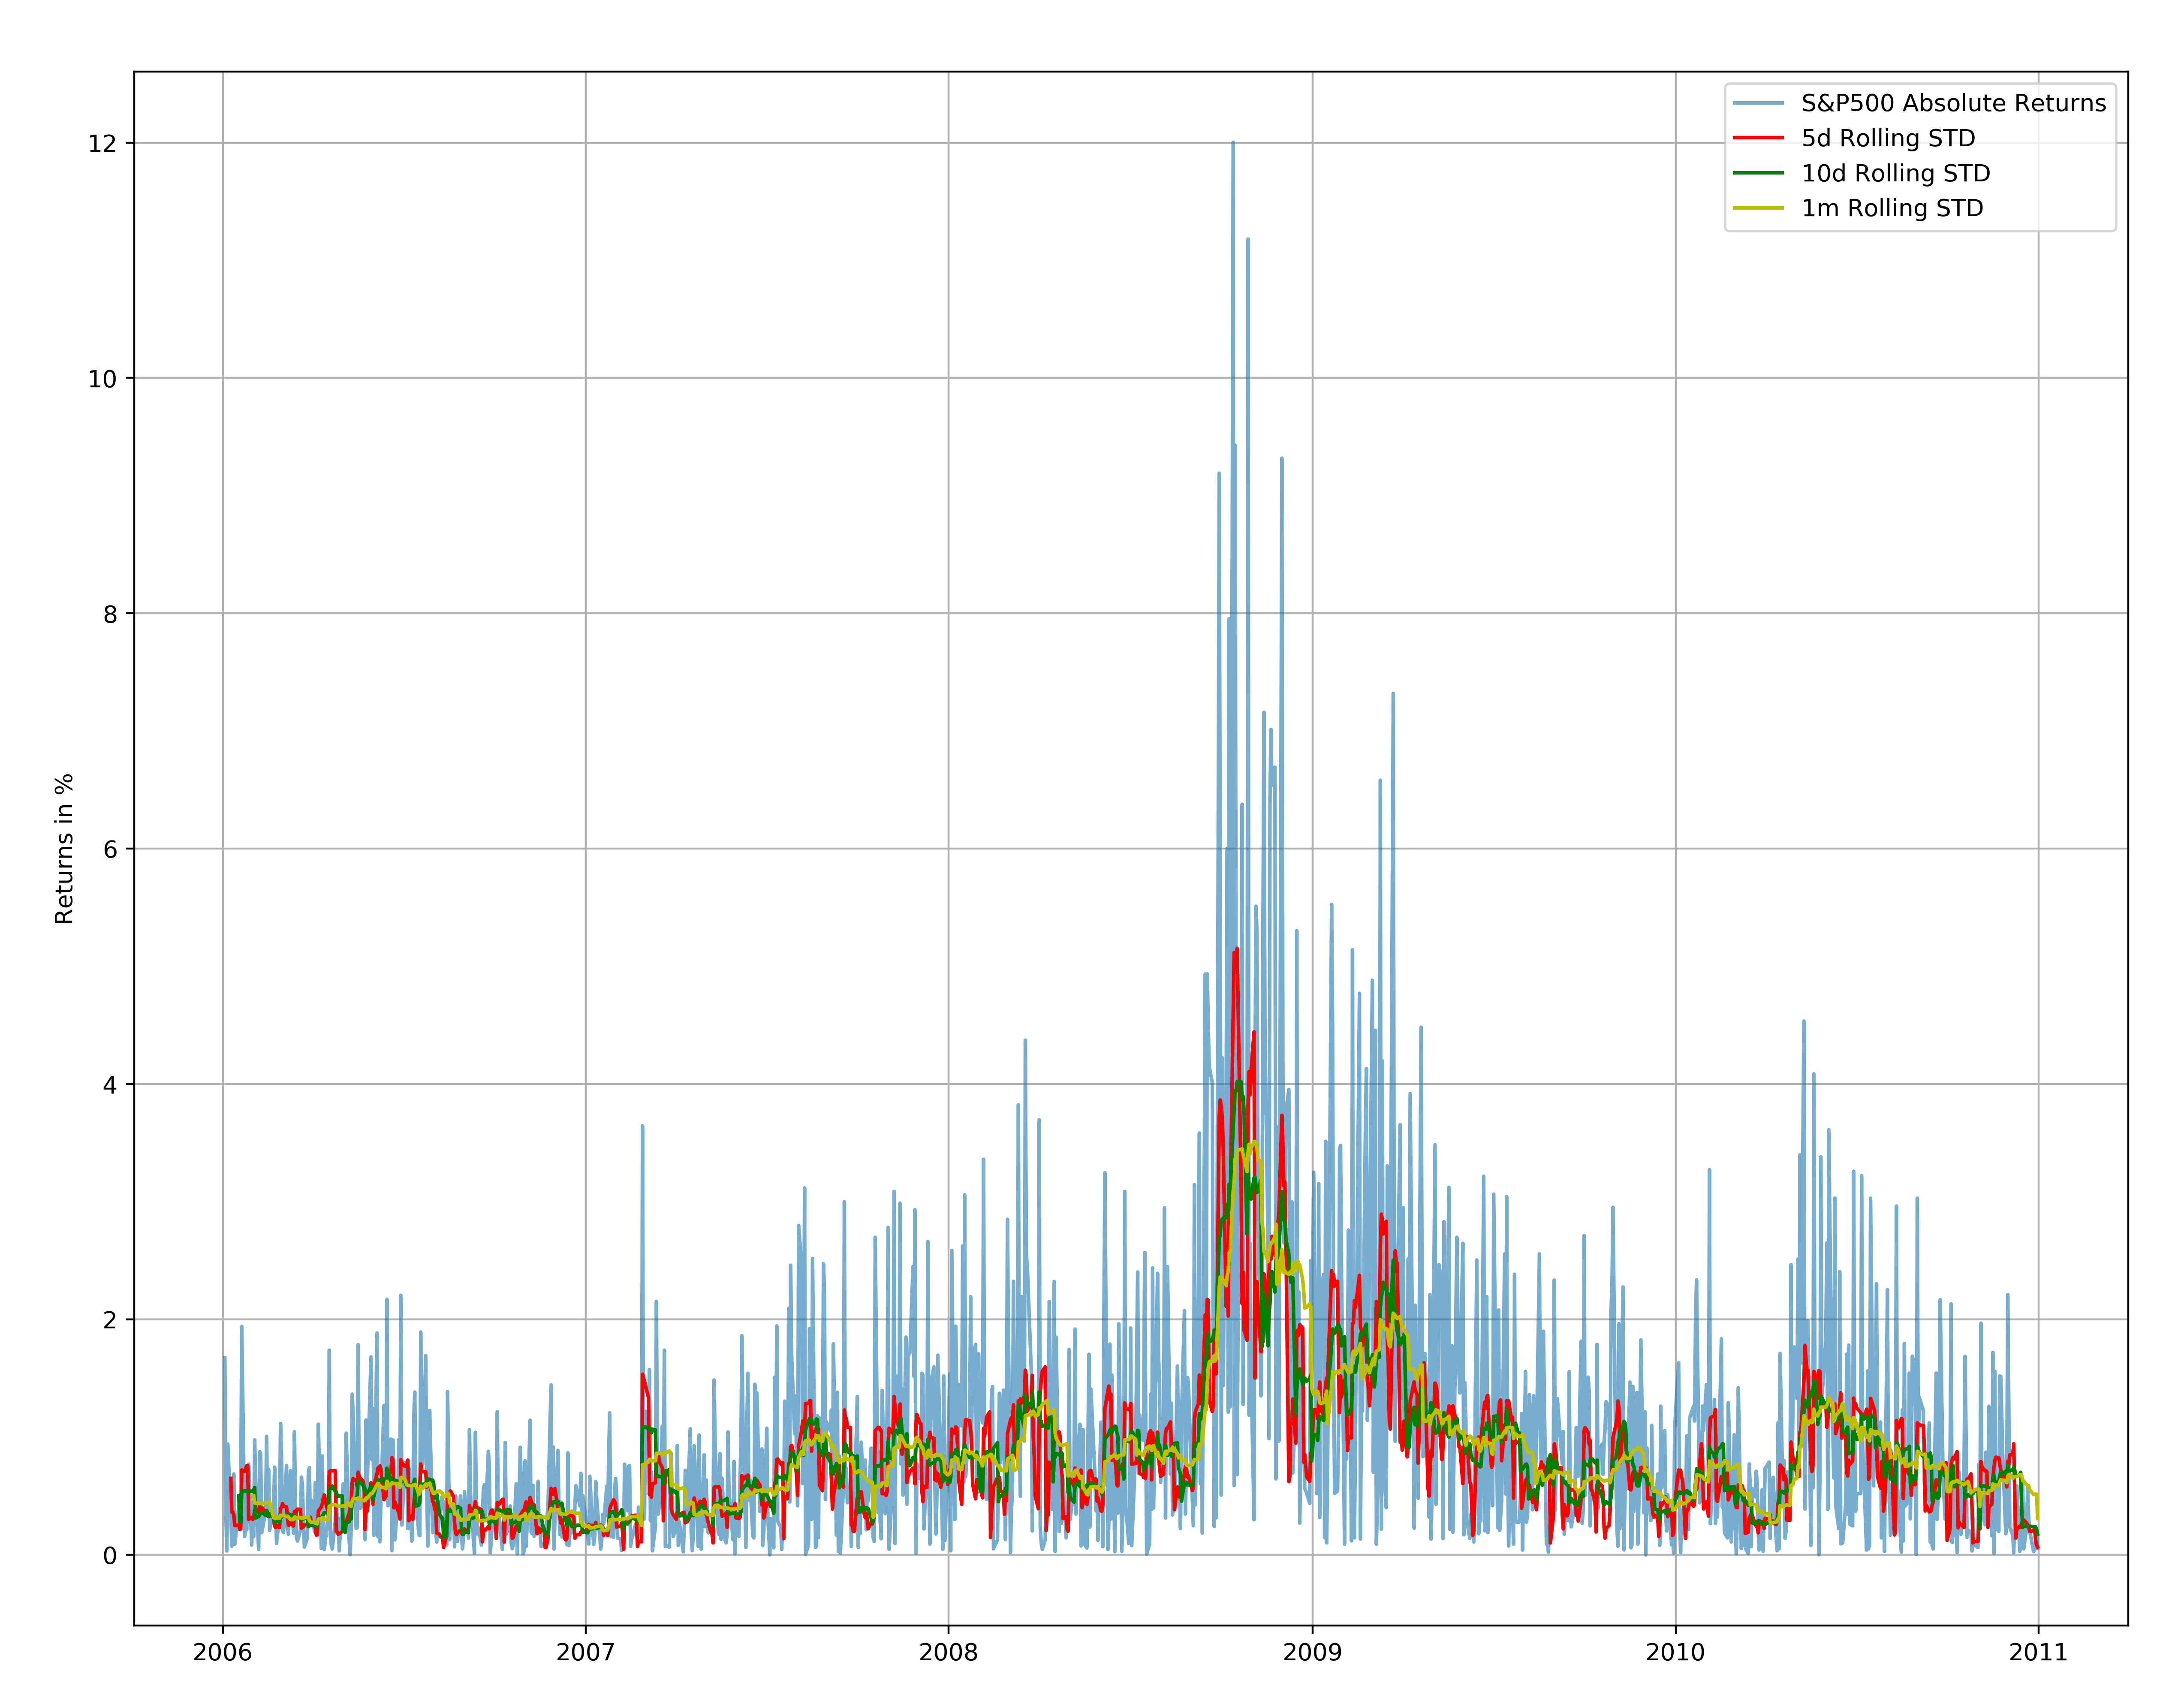
\includegraphics[width=\textwidth]{abs_sp500_returns.png}
\end{figure}
\end{frame}


\begin{frame}
\frametitle{Stylized Facts}
Further analysis of $\{X_t\}$ reveals other kinds of structure that cannot be explained by the gaussian assumption.\\
\vspace{0.5cm}
In particular, the return series displays the following distinctive behavior:

\begin{enumerate}
\item{$\{X_t\}$ is heavy-tailed, much more so than the Gaussian white noise}
\item{Although $\{X_t\}$ is uncorrelated, the series $\{X_{t}^2\}$ is highly correlated}
\item{The changes in $\{X_t\}$ tend to be clustered, large changes tend to be followed by large changes and vice v}
\item{Effects are asymmetric, bad news results in larger downward price moves than positive news does to upward price moves}
\end{enumerate}
\end{frame}

\begin{frame}
\frametitle{S&P500 Daily Returns (1950-2018)}
\begin{figure}[h!]
\centering 
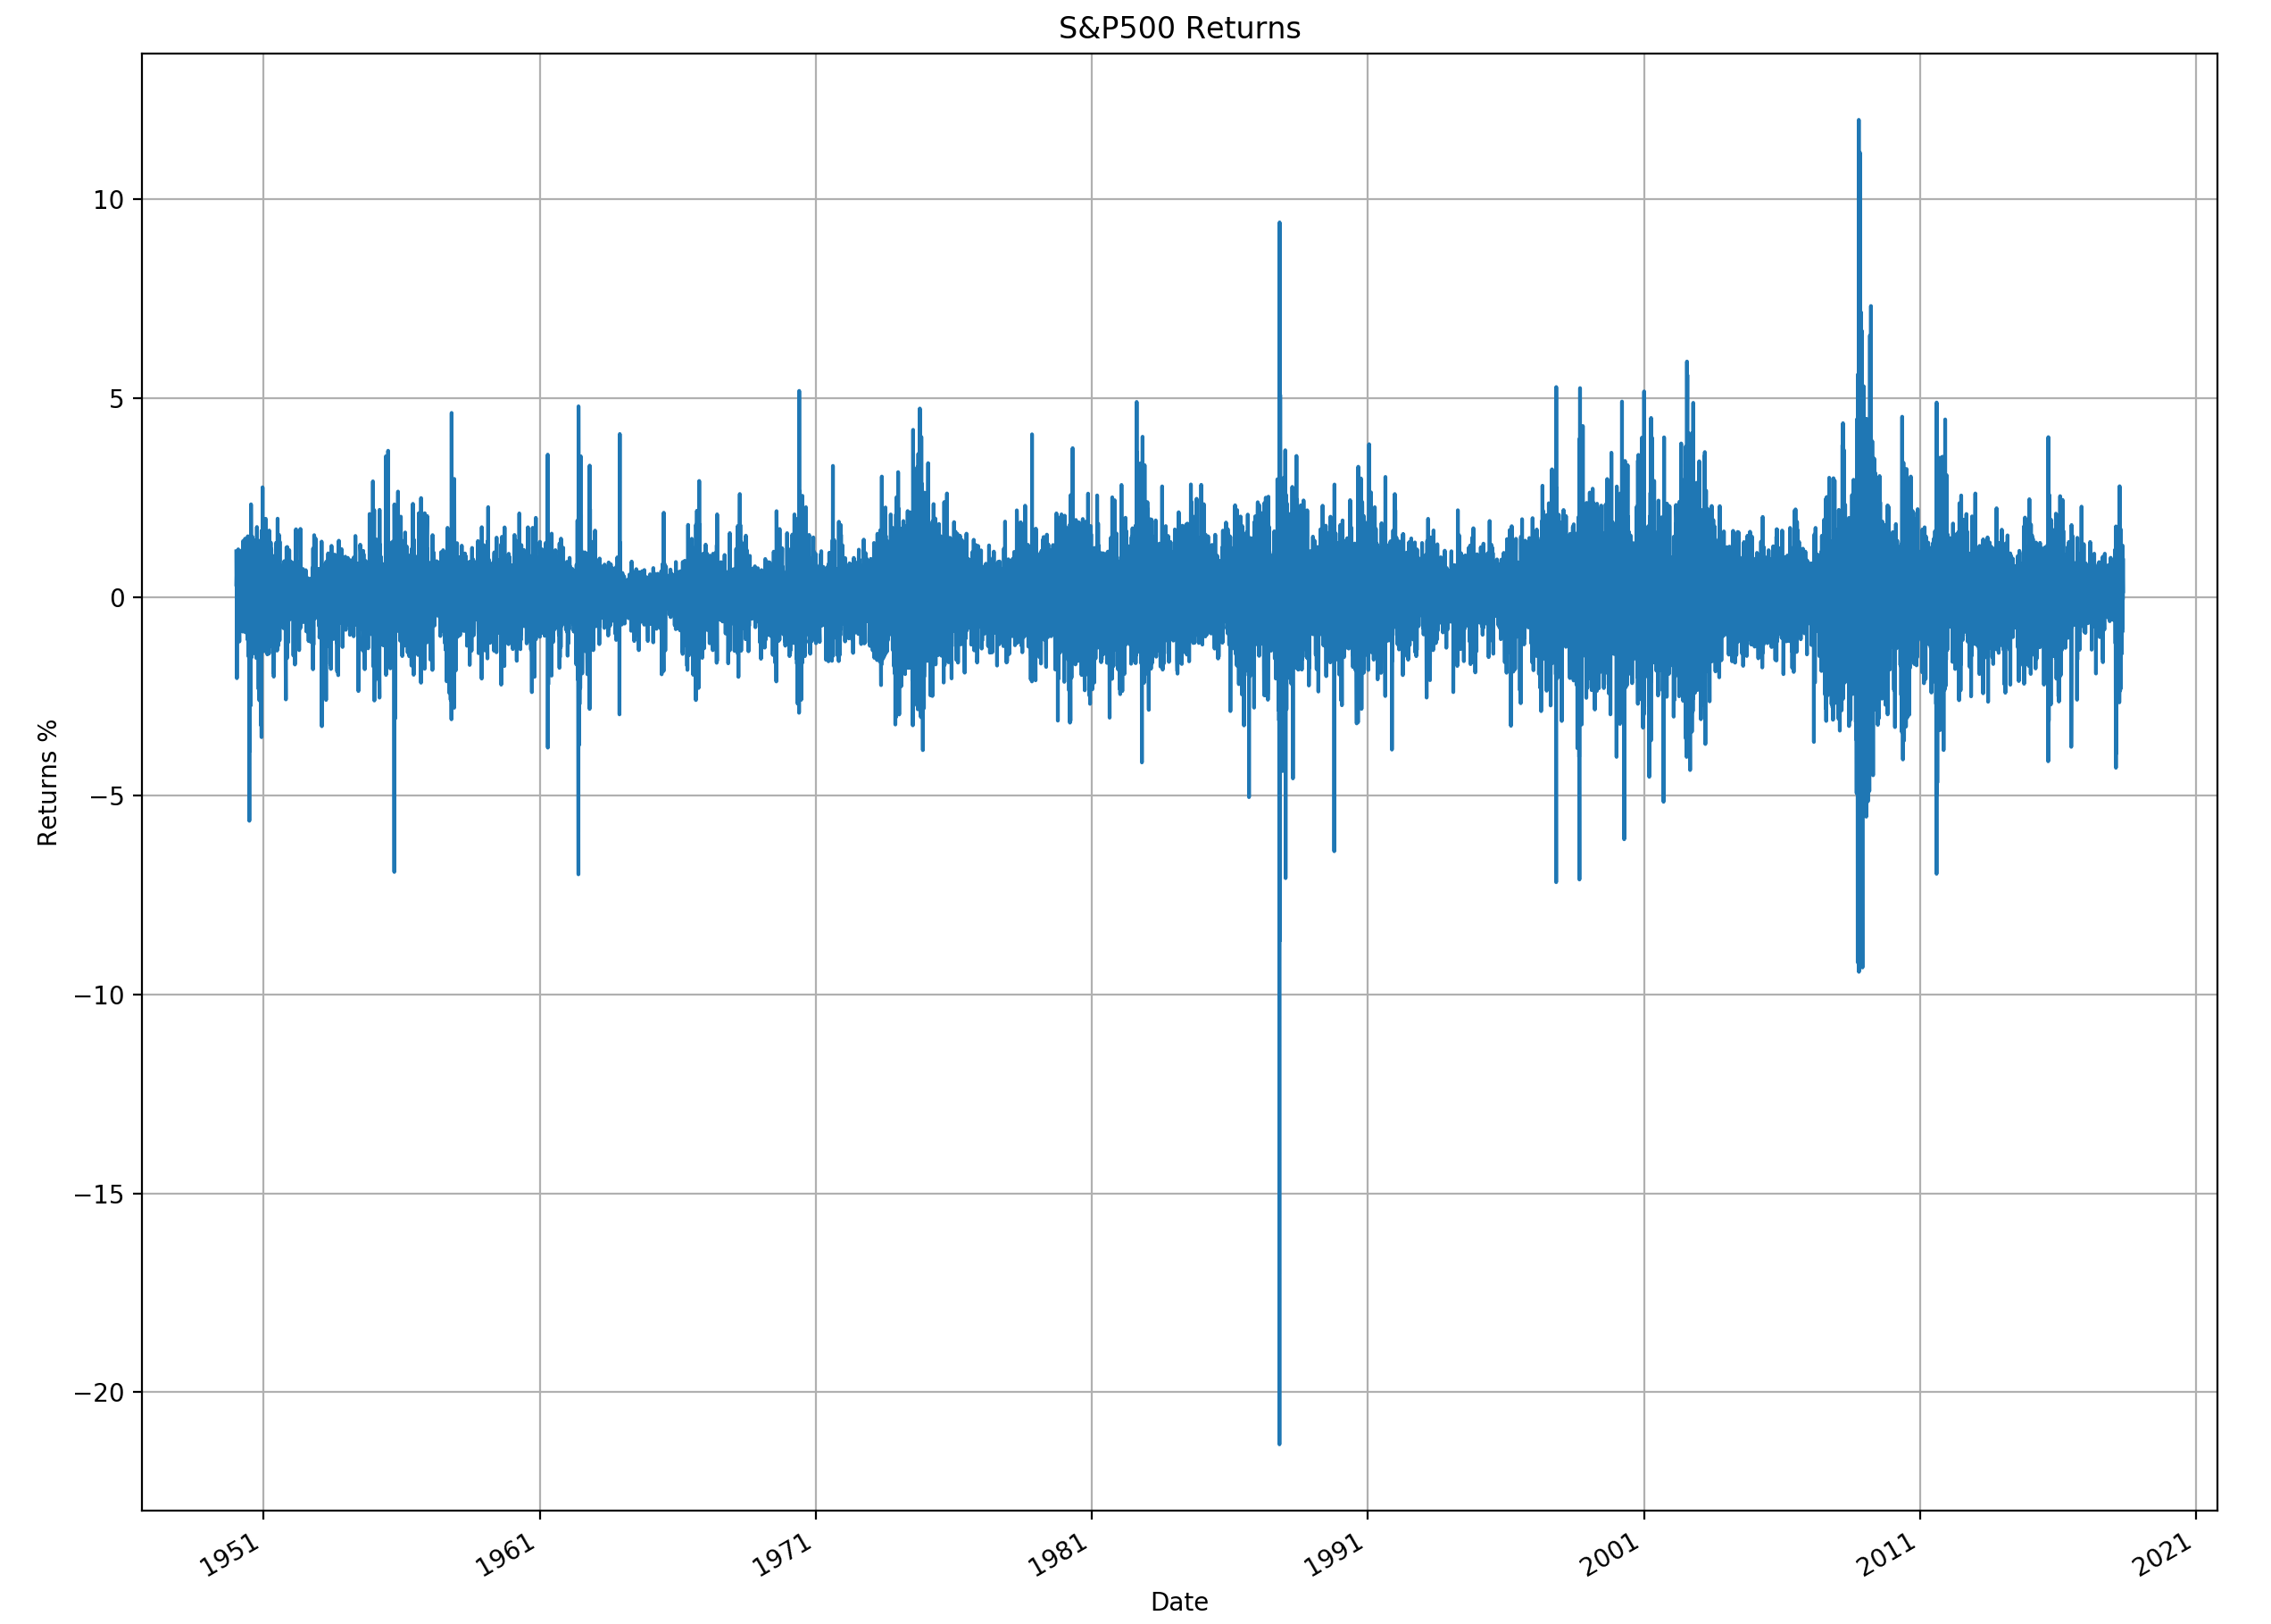
\includegraphics[width=\textwidth]{sp500_returns.png}
\end{figure}
\end{frame}


\begin{frame}
\frametitle{GARCH}
The Generalized ARCH (GARCH) model of Bollerslev (1986) and it's variants are extremely popular (albeit imperfect) methods to model volatility.\\
\vspace{15pt}
GARCH(p,q) model can be expressed as:

$$ X_t = \sigma_{t}\epsilon_{t}, \hspace{15pt} \epsilon_{t} \sim N(0,1) $$
where $$\sigma_{t}^{2} = \a_0 + \sum_{i=1}^{p} \beta_i \sigma_{t-i}^{2} + \sum_{j=1}^{q} \a_j X_{t-j}^{2}$$

For the purposes of this talk, we'll focus on GARCH(1,1) models where $\sigma_{t}^{2} = \a_0 + \beta_1 \sigma_{t-1}^{2} + \a_1 X_{t-1}^{2}$
\end{frame}

\section{Normalizing and Variance Stabilizing (NoVaS) Transformation}

\begin{frame}
\frametitle{Outline}
\tableofcontents[currentsection]
\end{frame}

\begin{frame}
\frametitle{NoVaS Transformation (Politis 2007)}
The NoVaS Transformation is defined as $$ W_{t,a} = \frac{X_t}{\sqrt{\alpha s^2_{t-1} + a_0 X^2_{t} + \sum_{i=1}^{p} a_i X^2_{t-i}}}$$ for $t=p+1,p+2,\dots,n$ \\
\vspace{3pt}
It is a clever extension of the ARCH model where we include the value $X_t$ in order to ``studentize'' the returns.\\
\vspace{5pt}
The order $p$ and the vector of nonnegative parameters $(\a,a_0,\dots,a_p)$ are chosen by the practitioner with the twin goals of normalization and variance-stabilization.\\
\vspace{5pt}
Algorithm for Simple NoVaS:
\begin{itemize}
\item{Let $\a = 0$ and $a_i = \frac{1}{p+1}$ for all $0 \leq i \leq p$}
\item{Pick $p$ such that $|KURT_{n}(W_{t,p}^{S})| \approx 3$}
\end{itemize}




\end{frame}


%% S&P 500 %%
\begin{frame}
\frametitle{S&P500 Daily Returns (1950-2018)}
\begin{figure}[h!]
\centering 
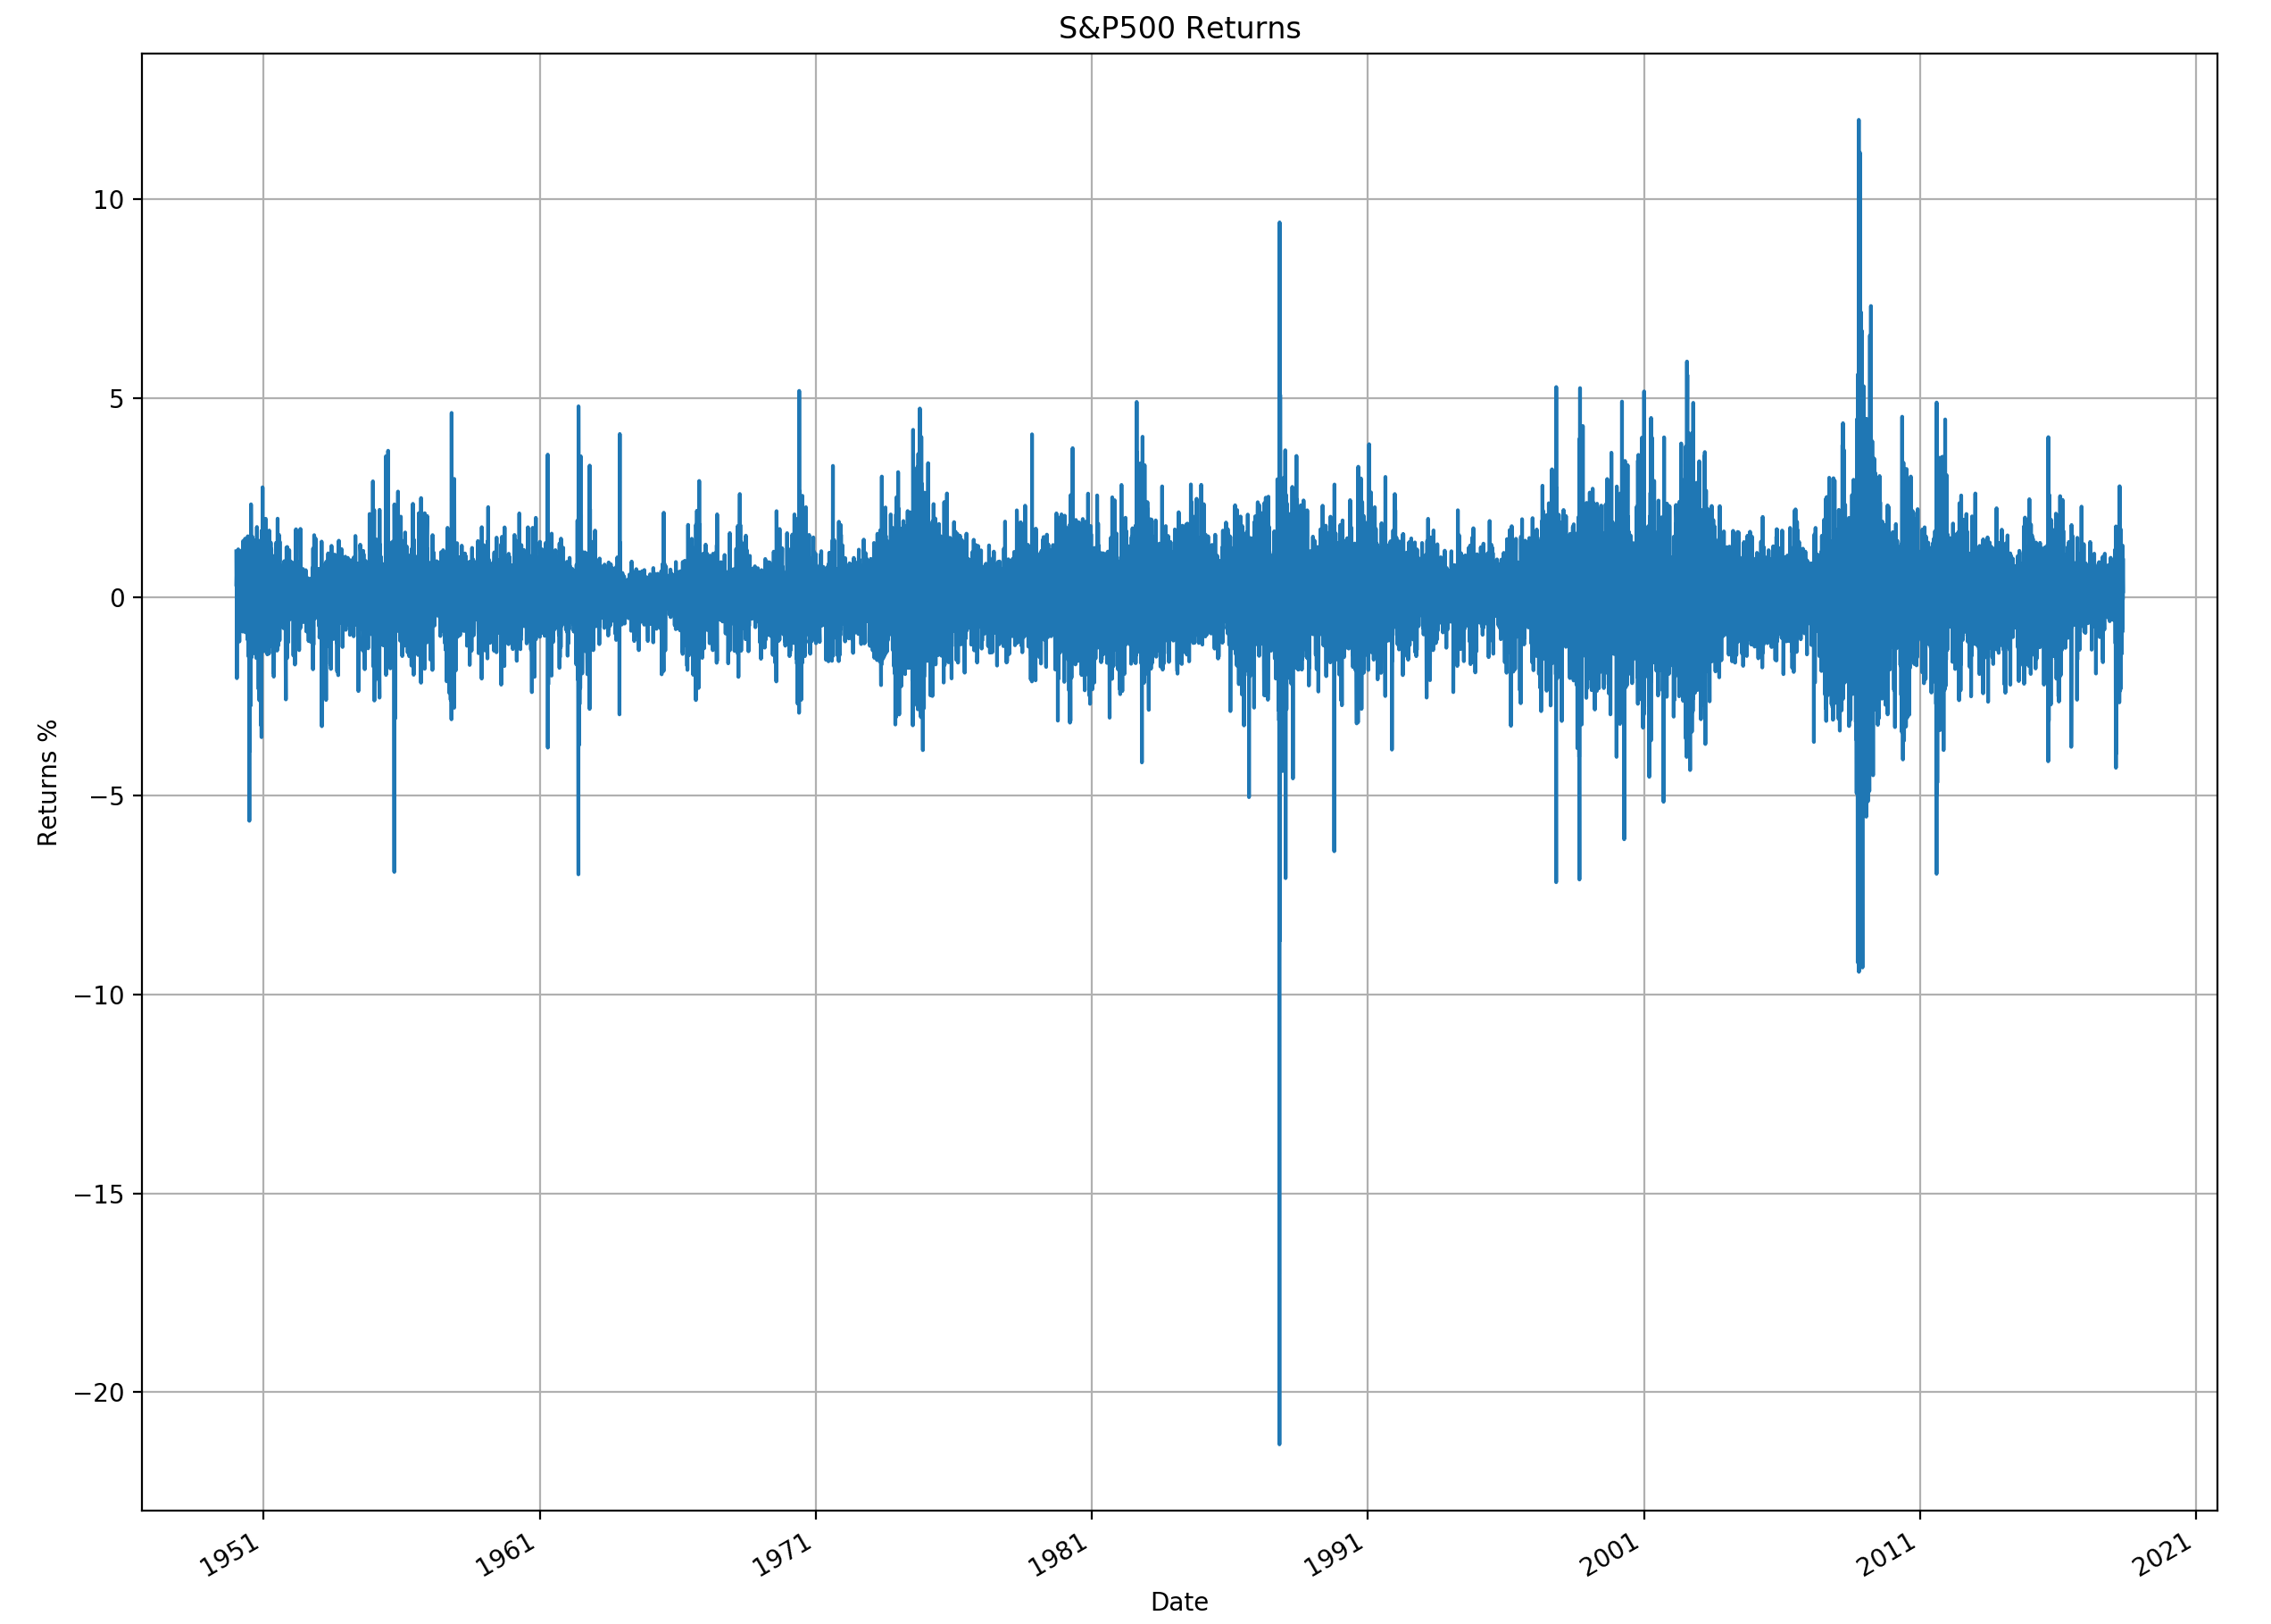
\includegraphics[width=\textwidth]{sp500_returns.png}
\end{figure}
\end{frame}

\begin{frame}
\frametitle{S&P500 Daily Returns Histogram}
\begin{figure}[h!]
\centering 
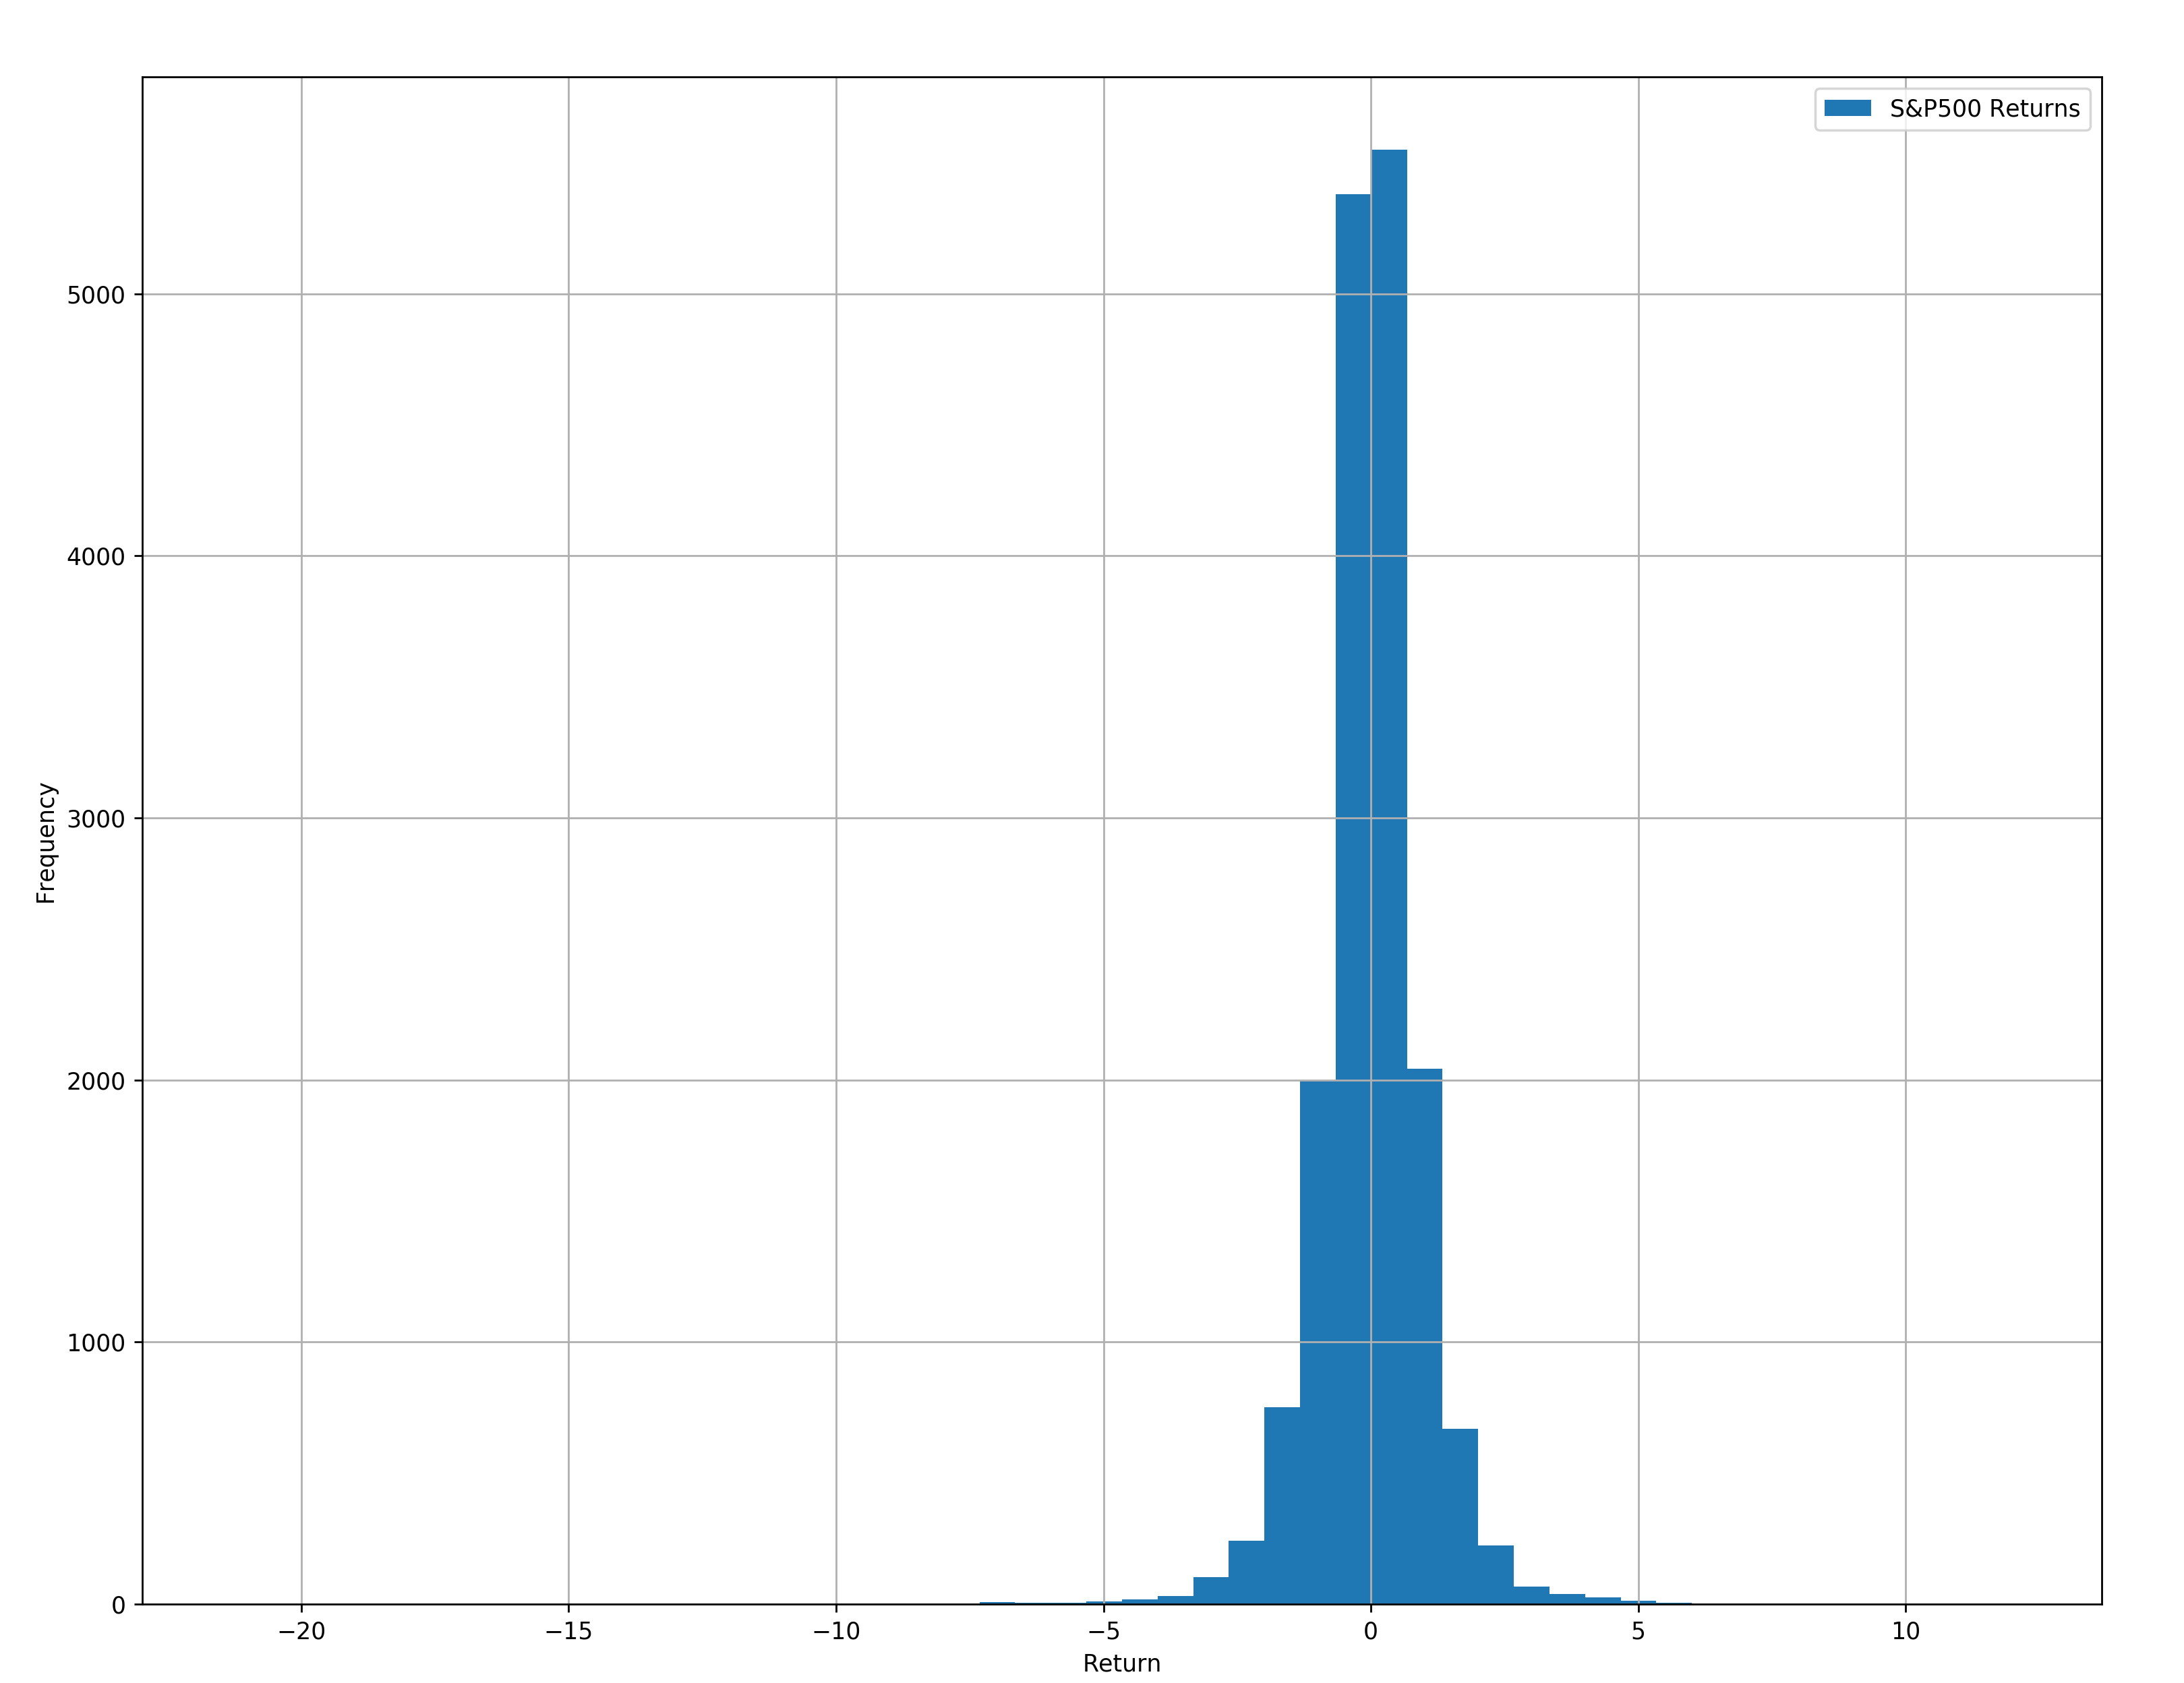
\includegraphics[width=\textwidth]{sp500_returns_hist.png}
\end{figure}
\end{frame}

\begin{frame}
\frametitle{S&P500 Daily Returns Q-Q Plot}
\begin{figure}[h!]
\centering 
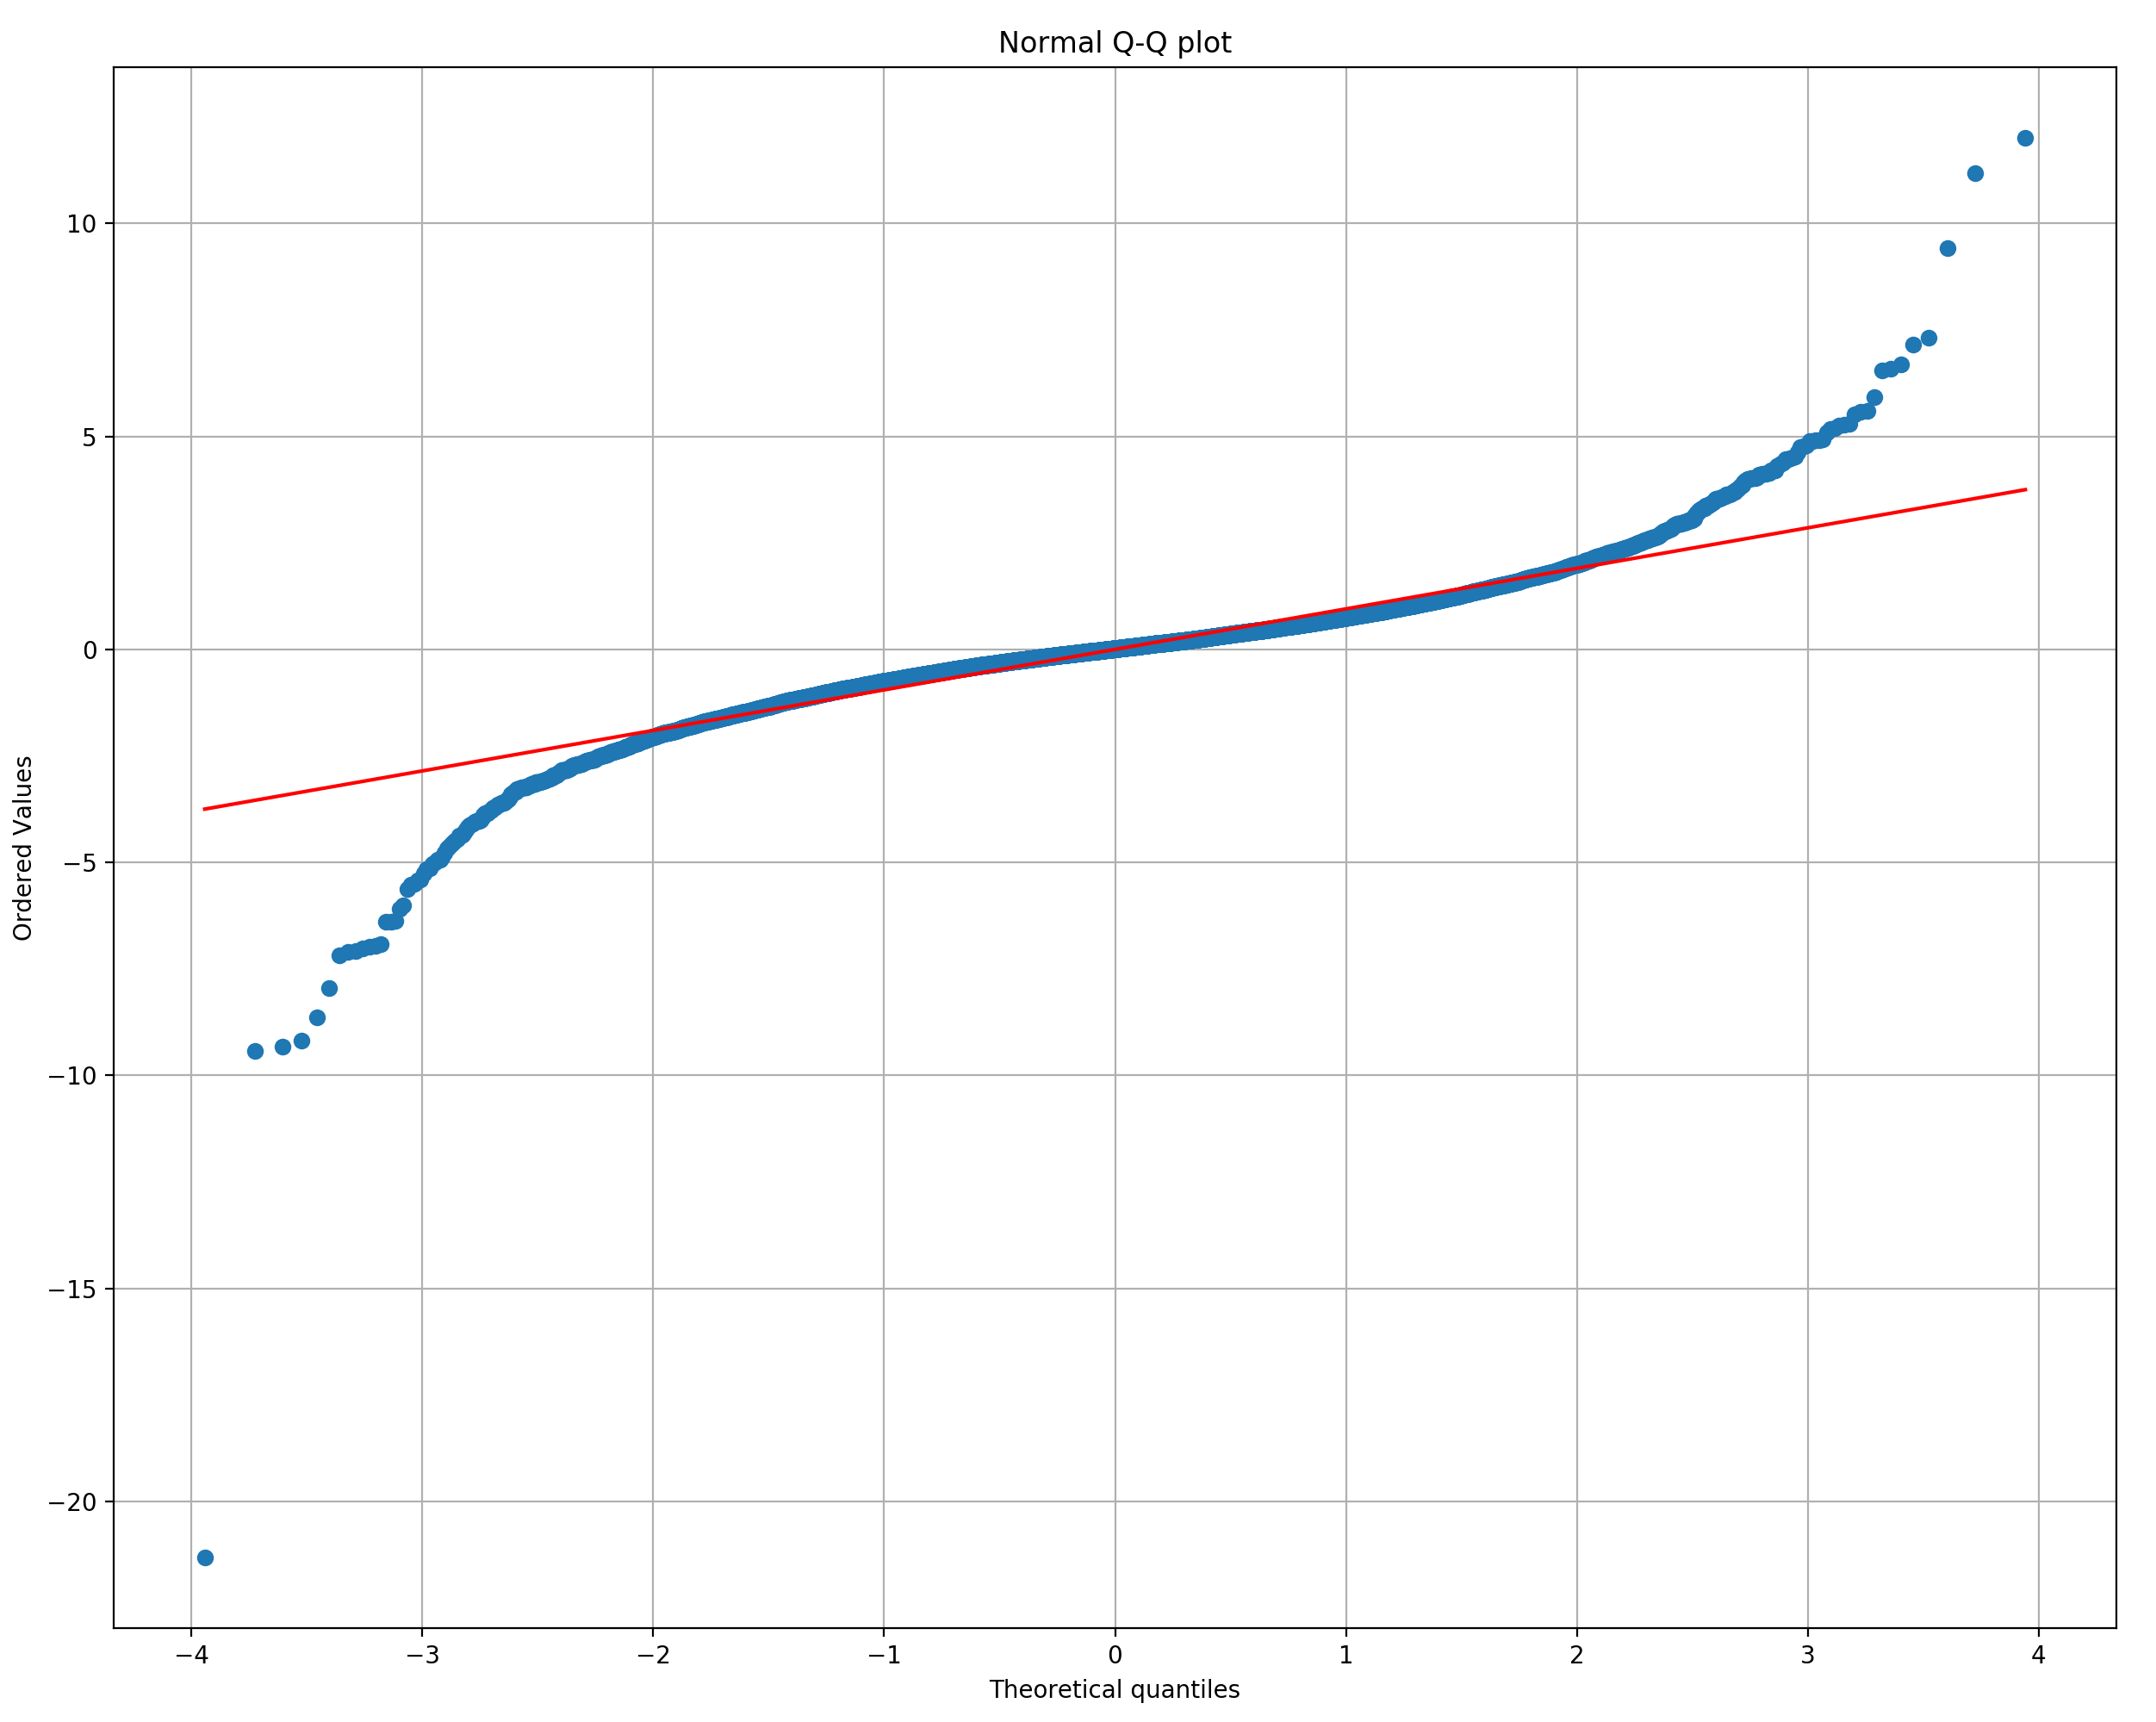
\includegraphics[width=\textwidth]{sp500_returns_qqplot.png}
\end{figure}
\end{frame}

\begin{frame}
\frametitle{NoVaS Transformed S&P500 Daily Returns (p=16)}
\begin{figure}[h!]
\centering 
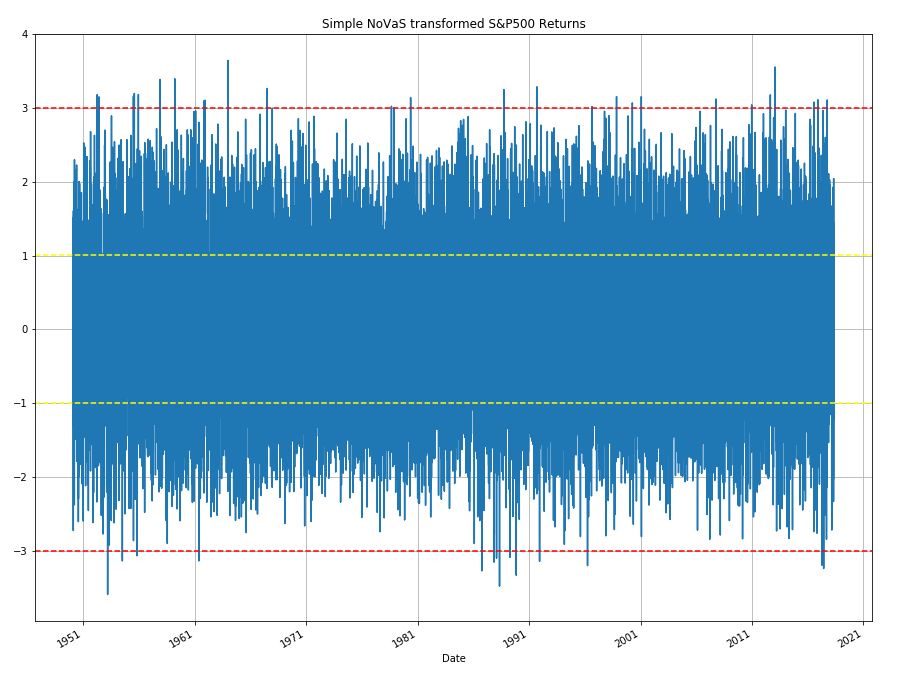
\includegraphics[width=\textwidth]{novas_sp500_returns.png}
\end{figure}
\end{frame}

\begin{frame}
\frametitle{NoVaS Transformed S&P500 Histogram (p=16)}
\begin{figure}[h!]
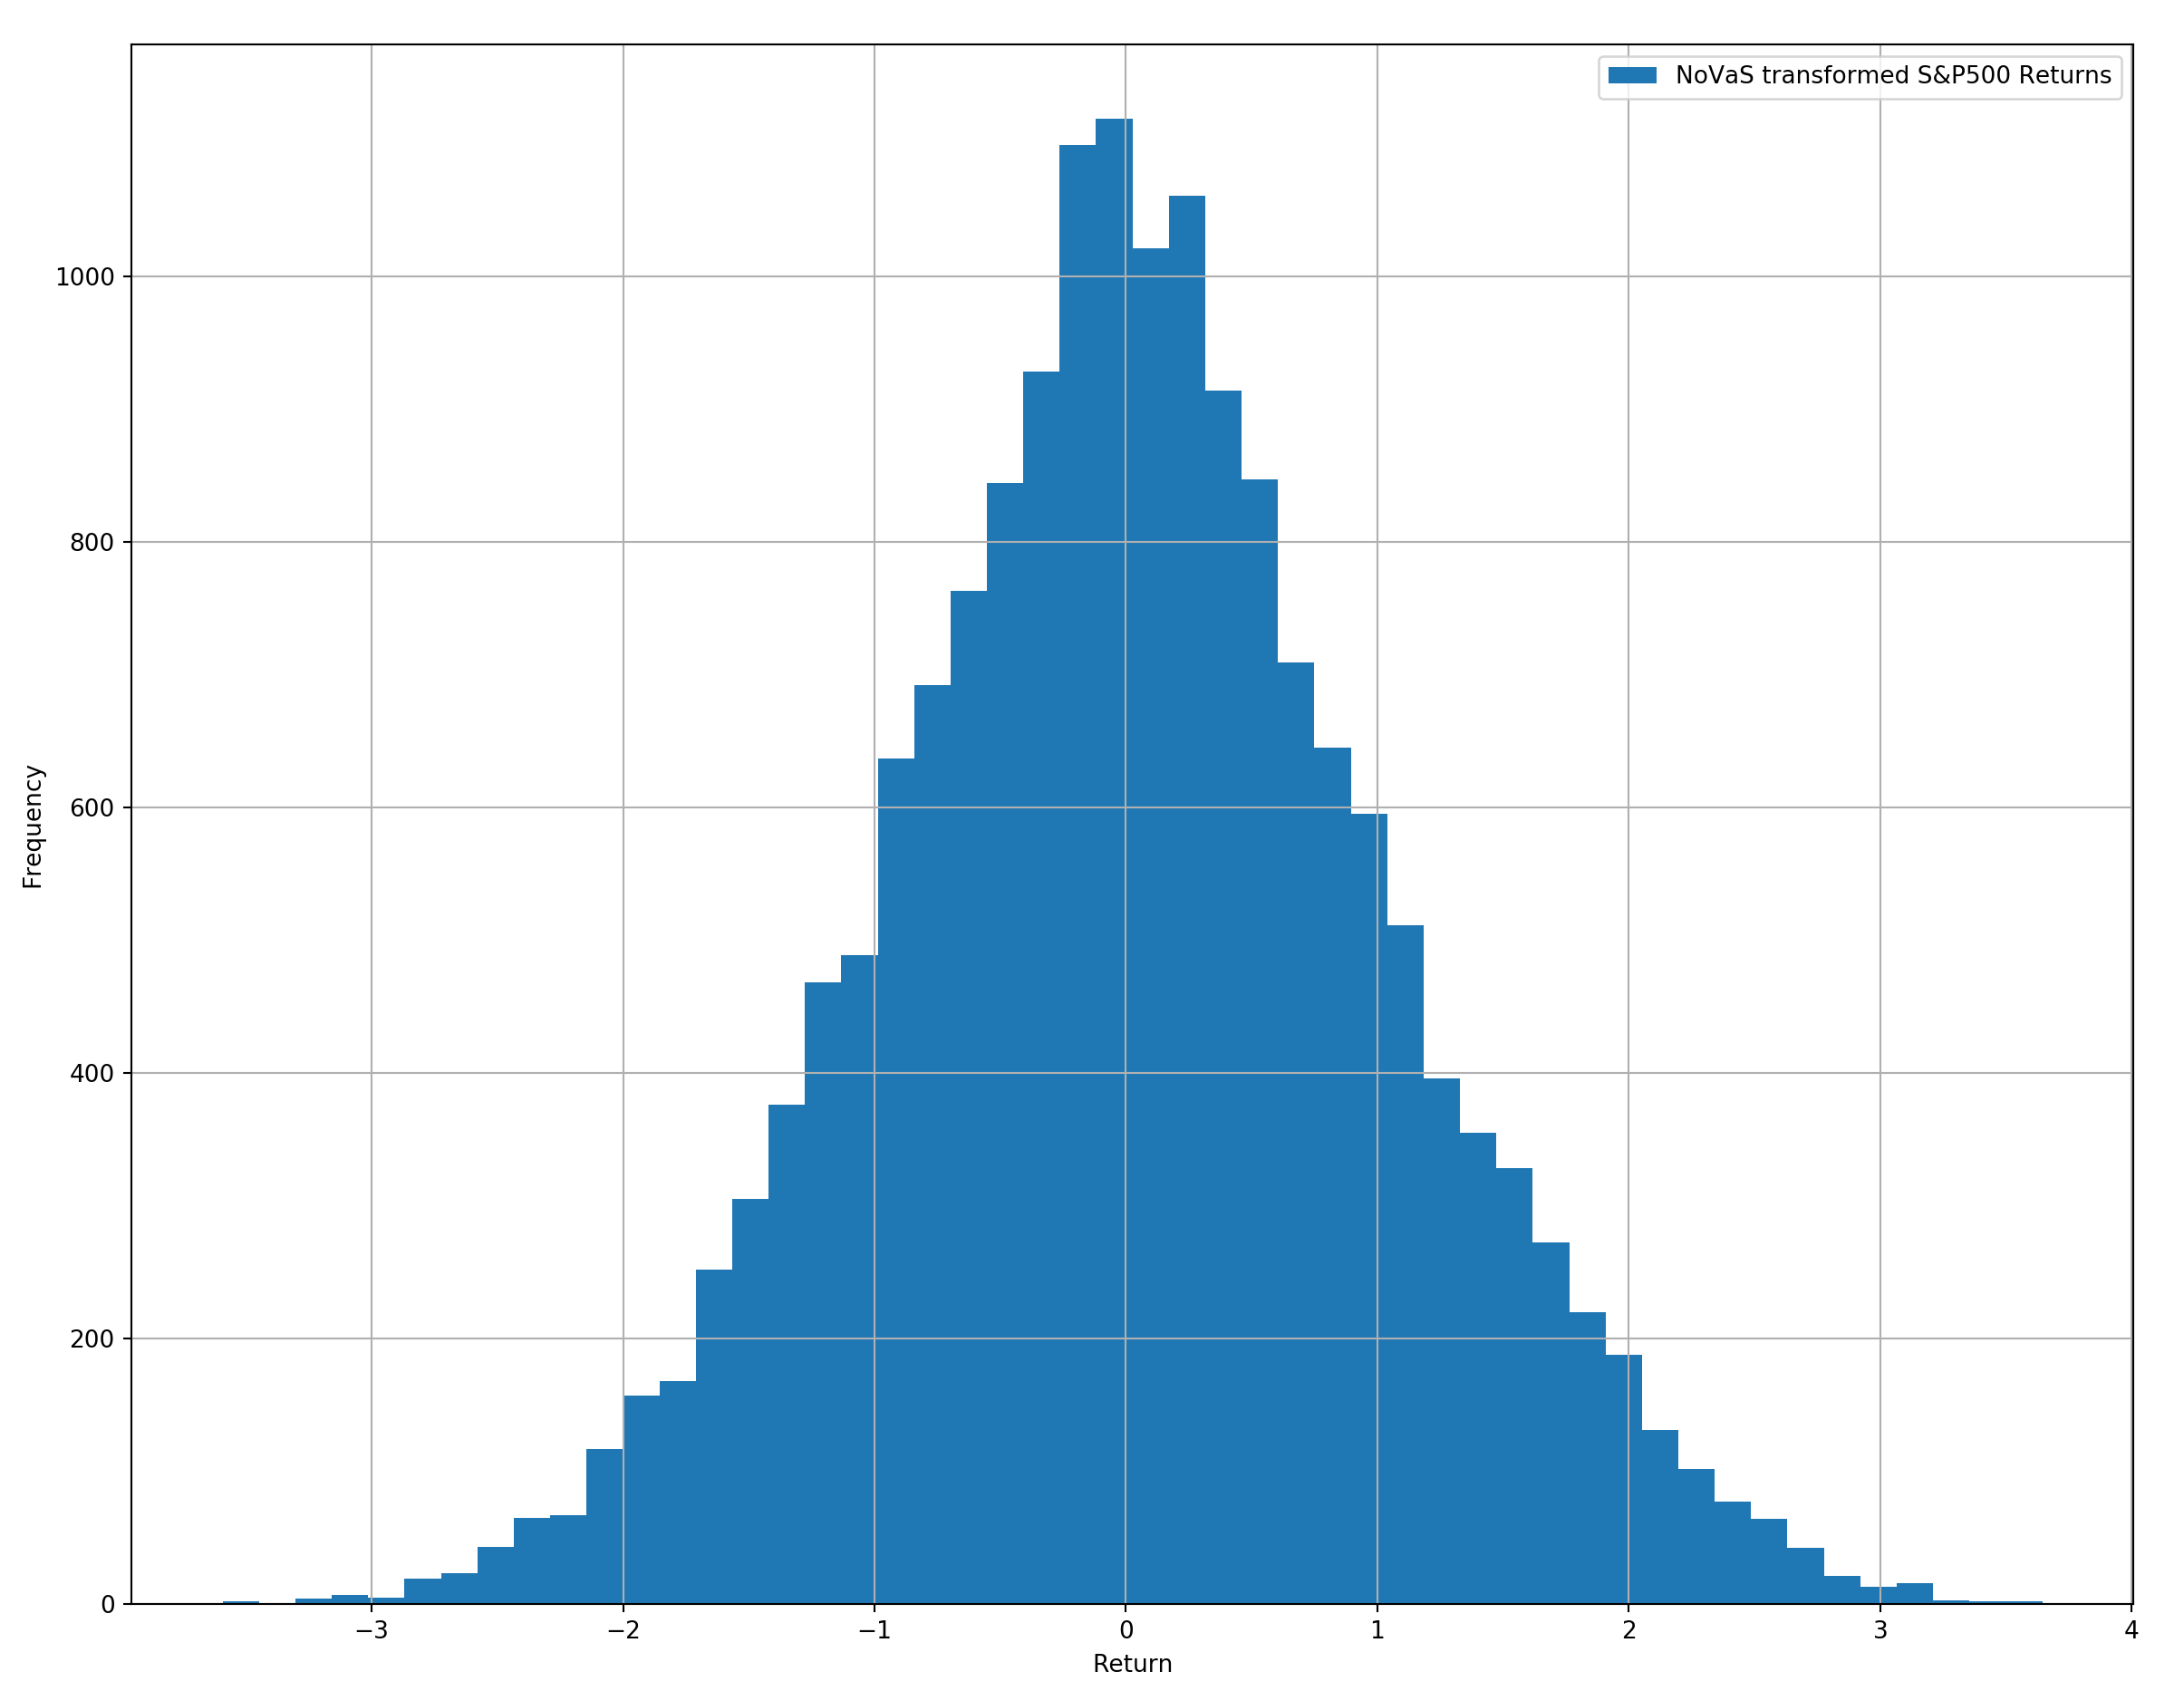
\includegraphics[width=\textwidth]{novas_sp500_returns_hist.png}
\end{figure}
\end{frame}

\begin{frame}
\frametitle{NoVaS Transformed S&P500 QQ-Plot (p=16)}
\begin{figure}[h!]
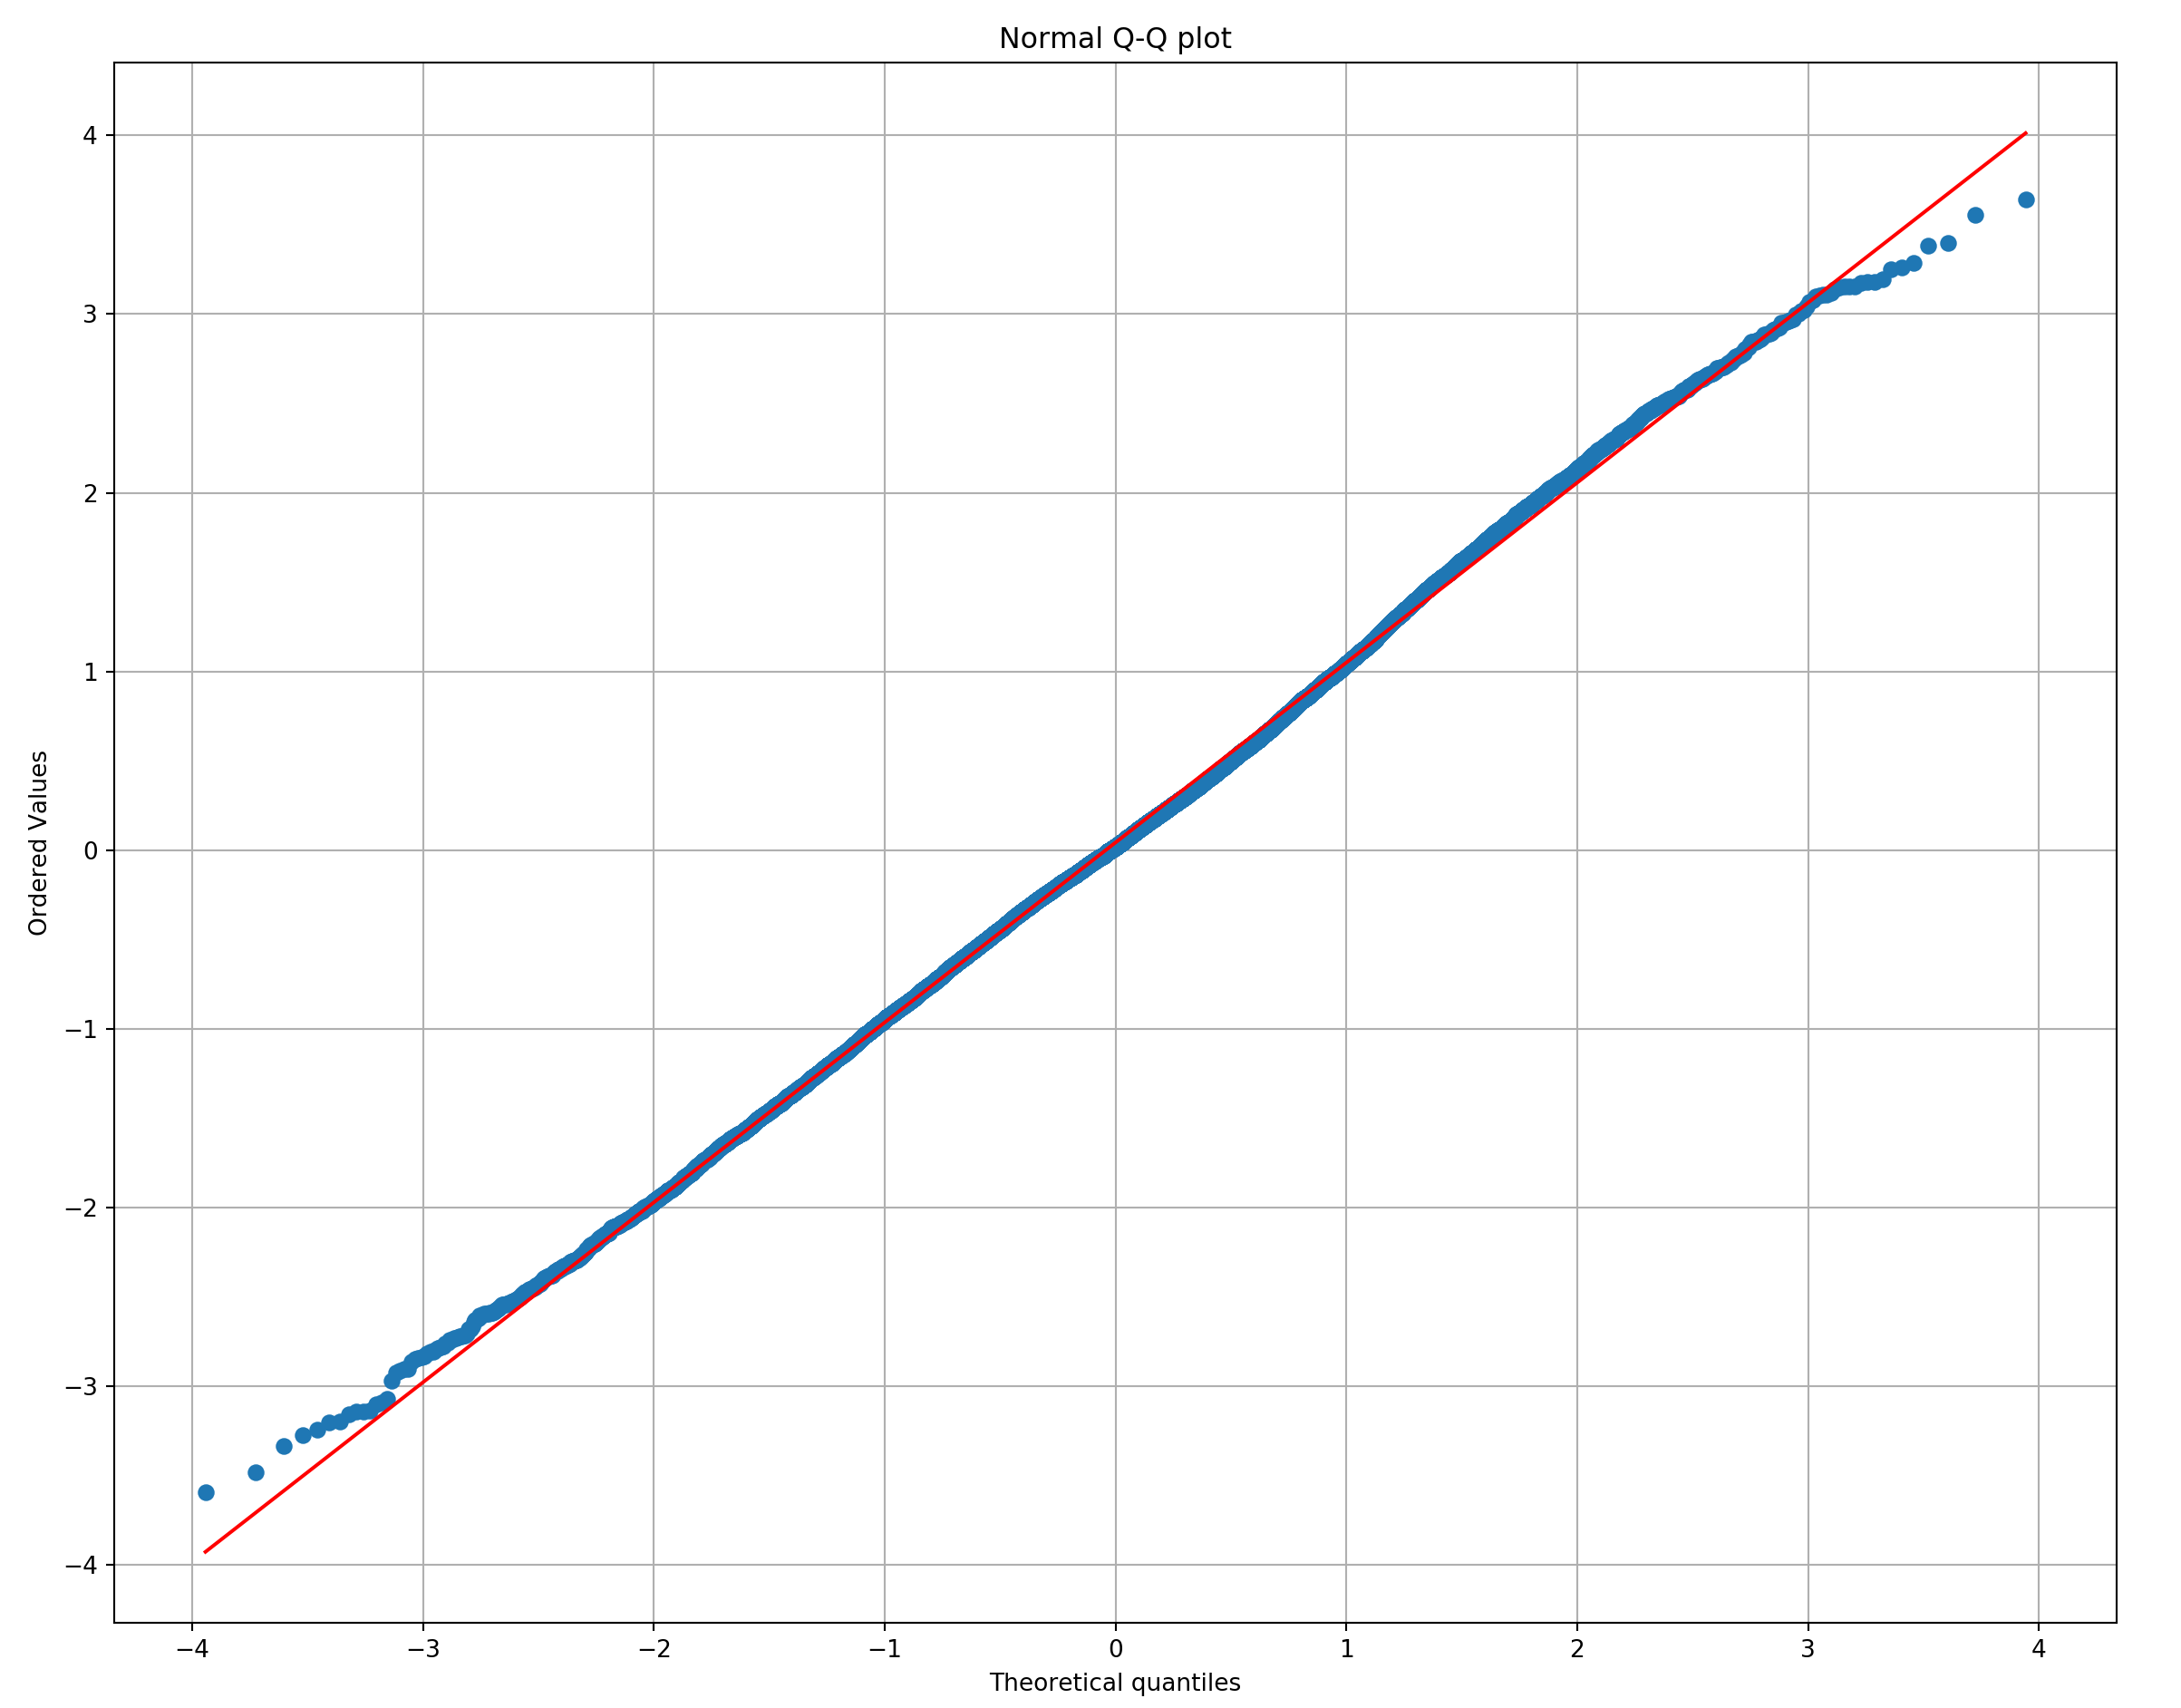
\includegraphics[width=\textwidth]{novas_sp500_returns_qqplot.png}
\end{figure}
\end{frame}

%%%%%%%%%%%%%%%%%%%
%%%%%%% BTC %%%%%%%
%%%%%%%%%%%%%%%%%%%

\begin{frame}
\frametitle{BTC/USD Daily Returns (2010-2018)}
\begin{figure}[h!]
\centering 
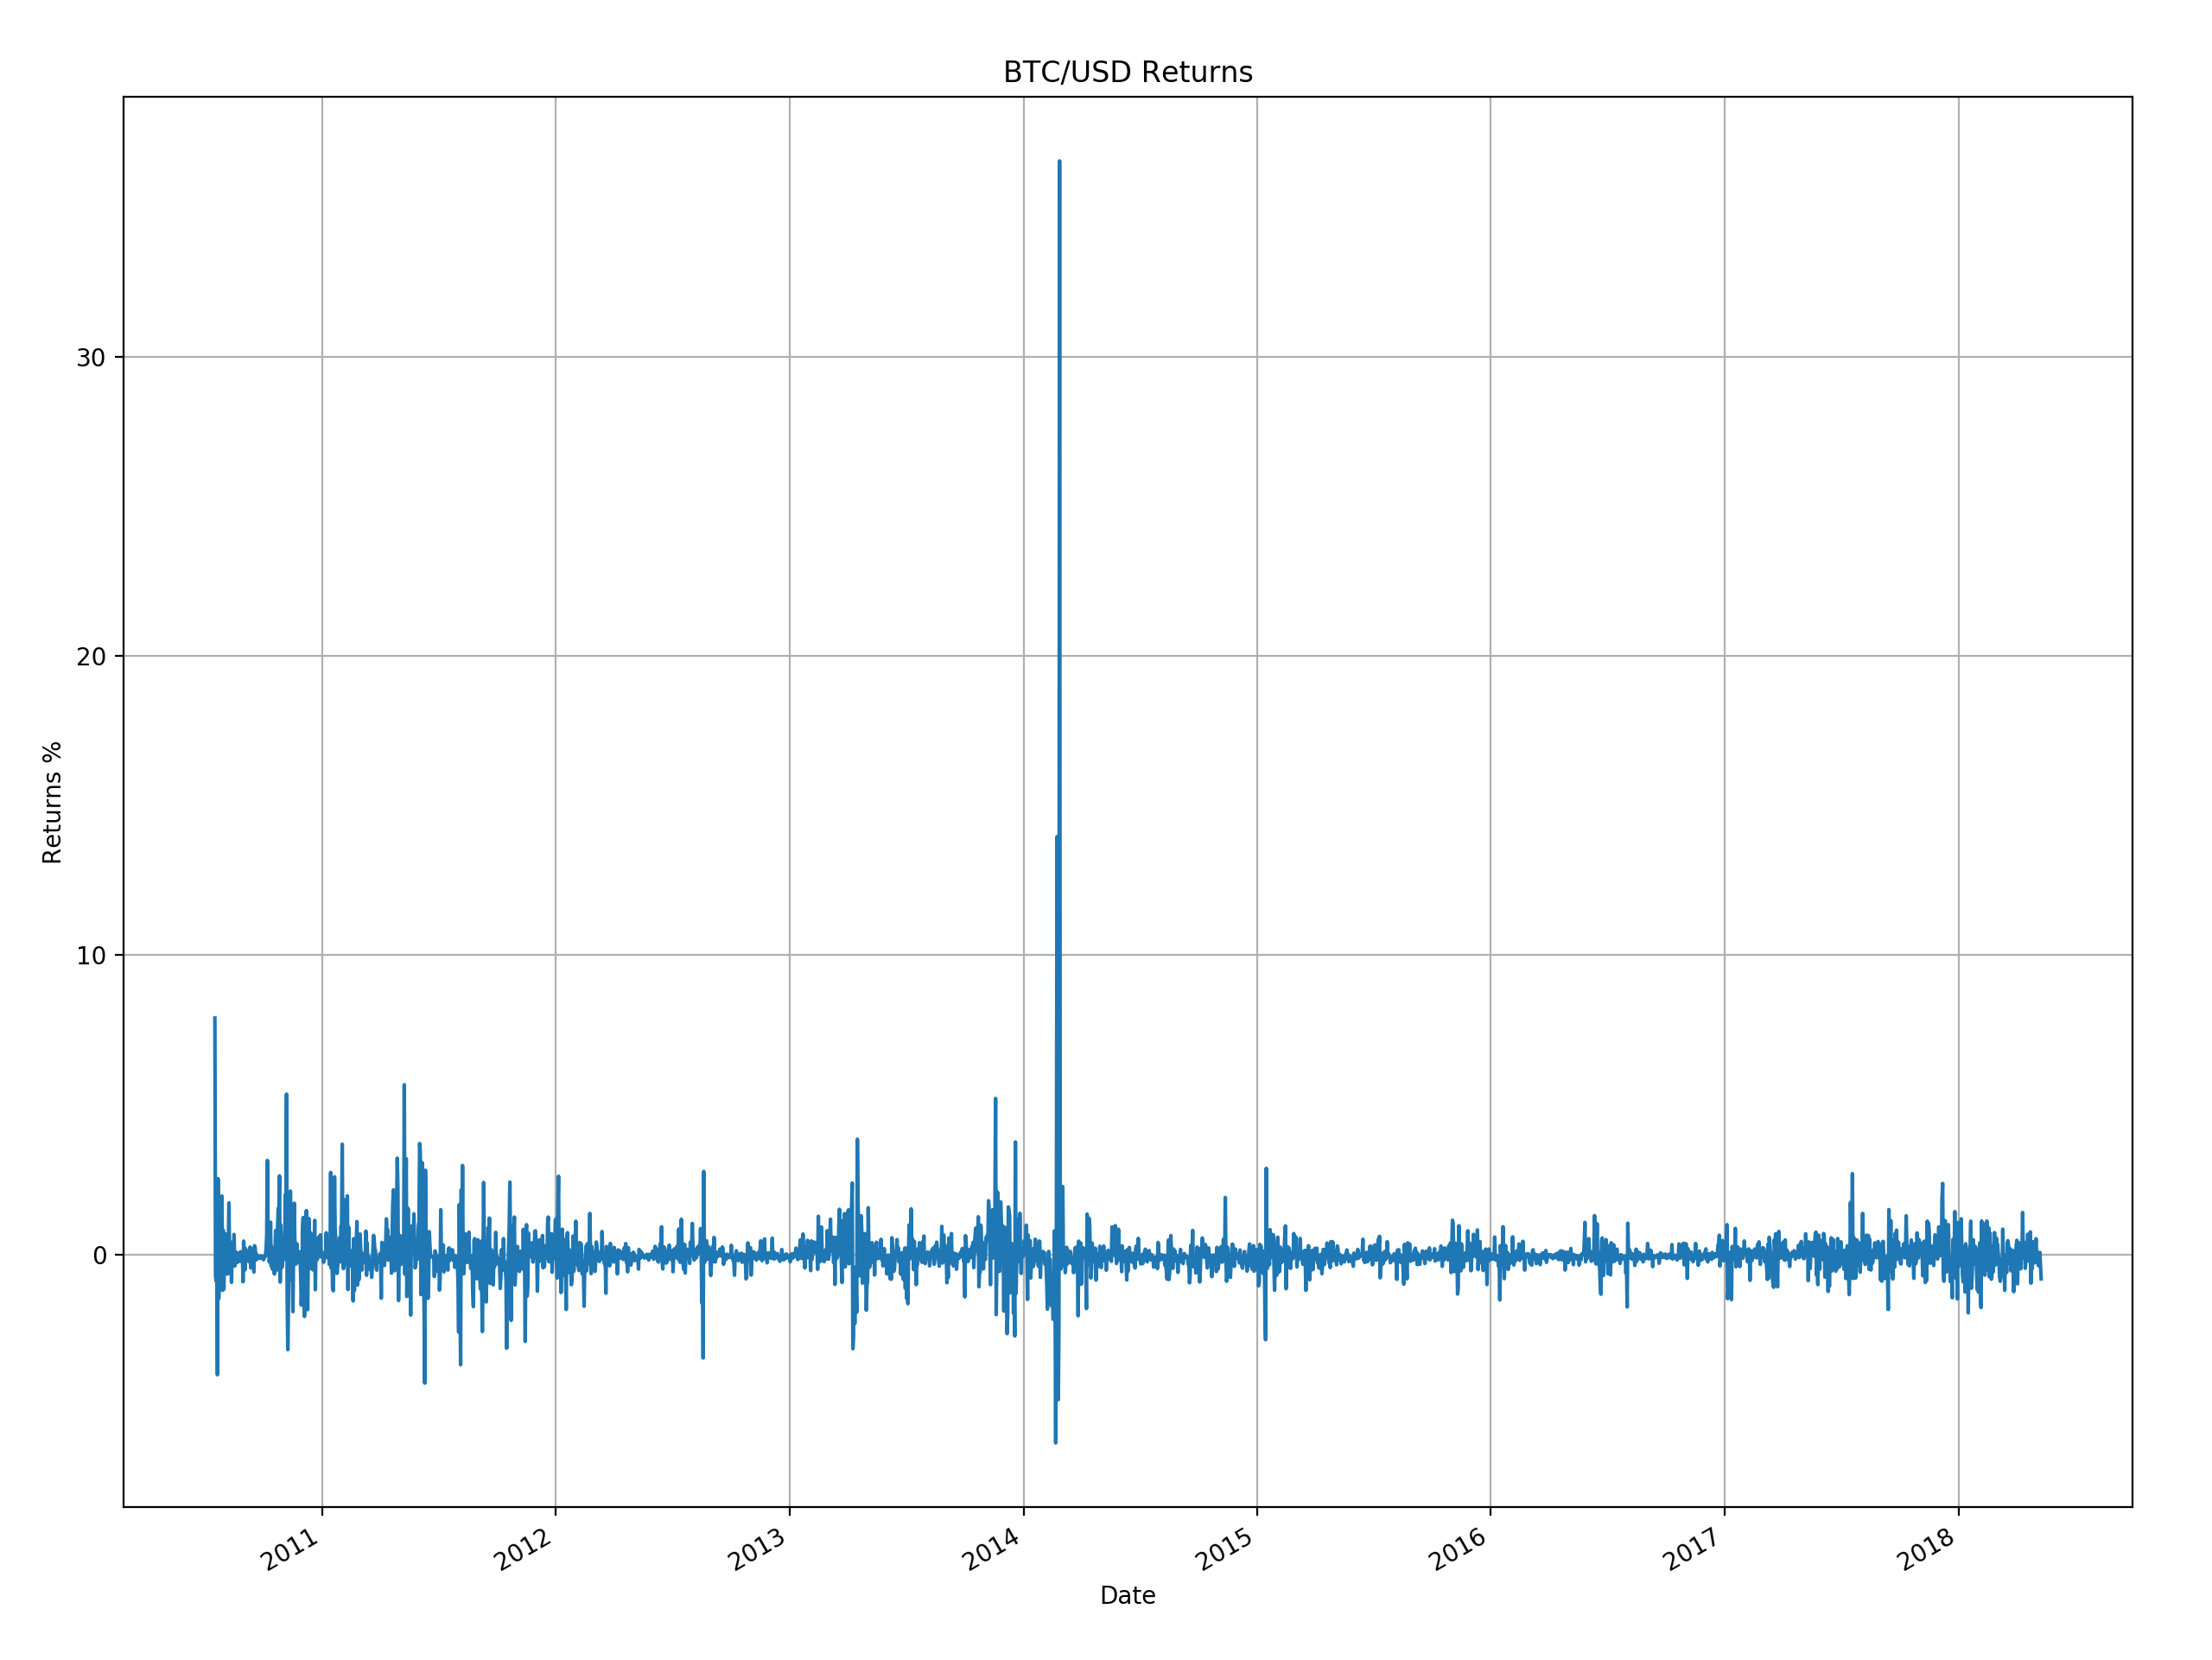
\includegraphics[width=\textwidth]{btc_returns.png}
\end{figure}
\end{frame}

\begin{frame}
\frametitle{BTC/USD Daily Returns Histogram (2010-2018)}
\begin{figure}[h!]
\centering 
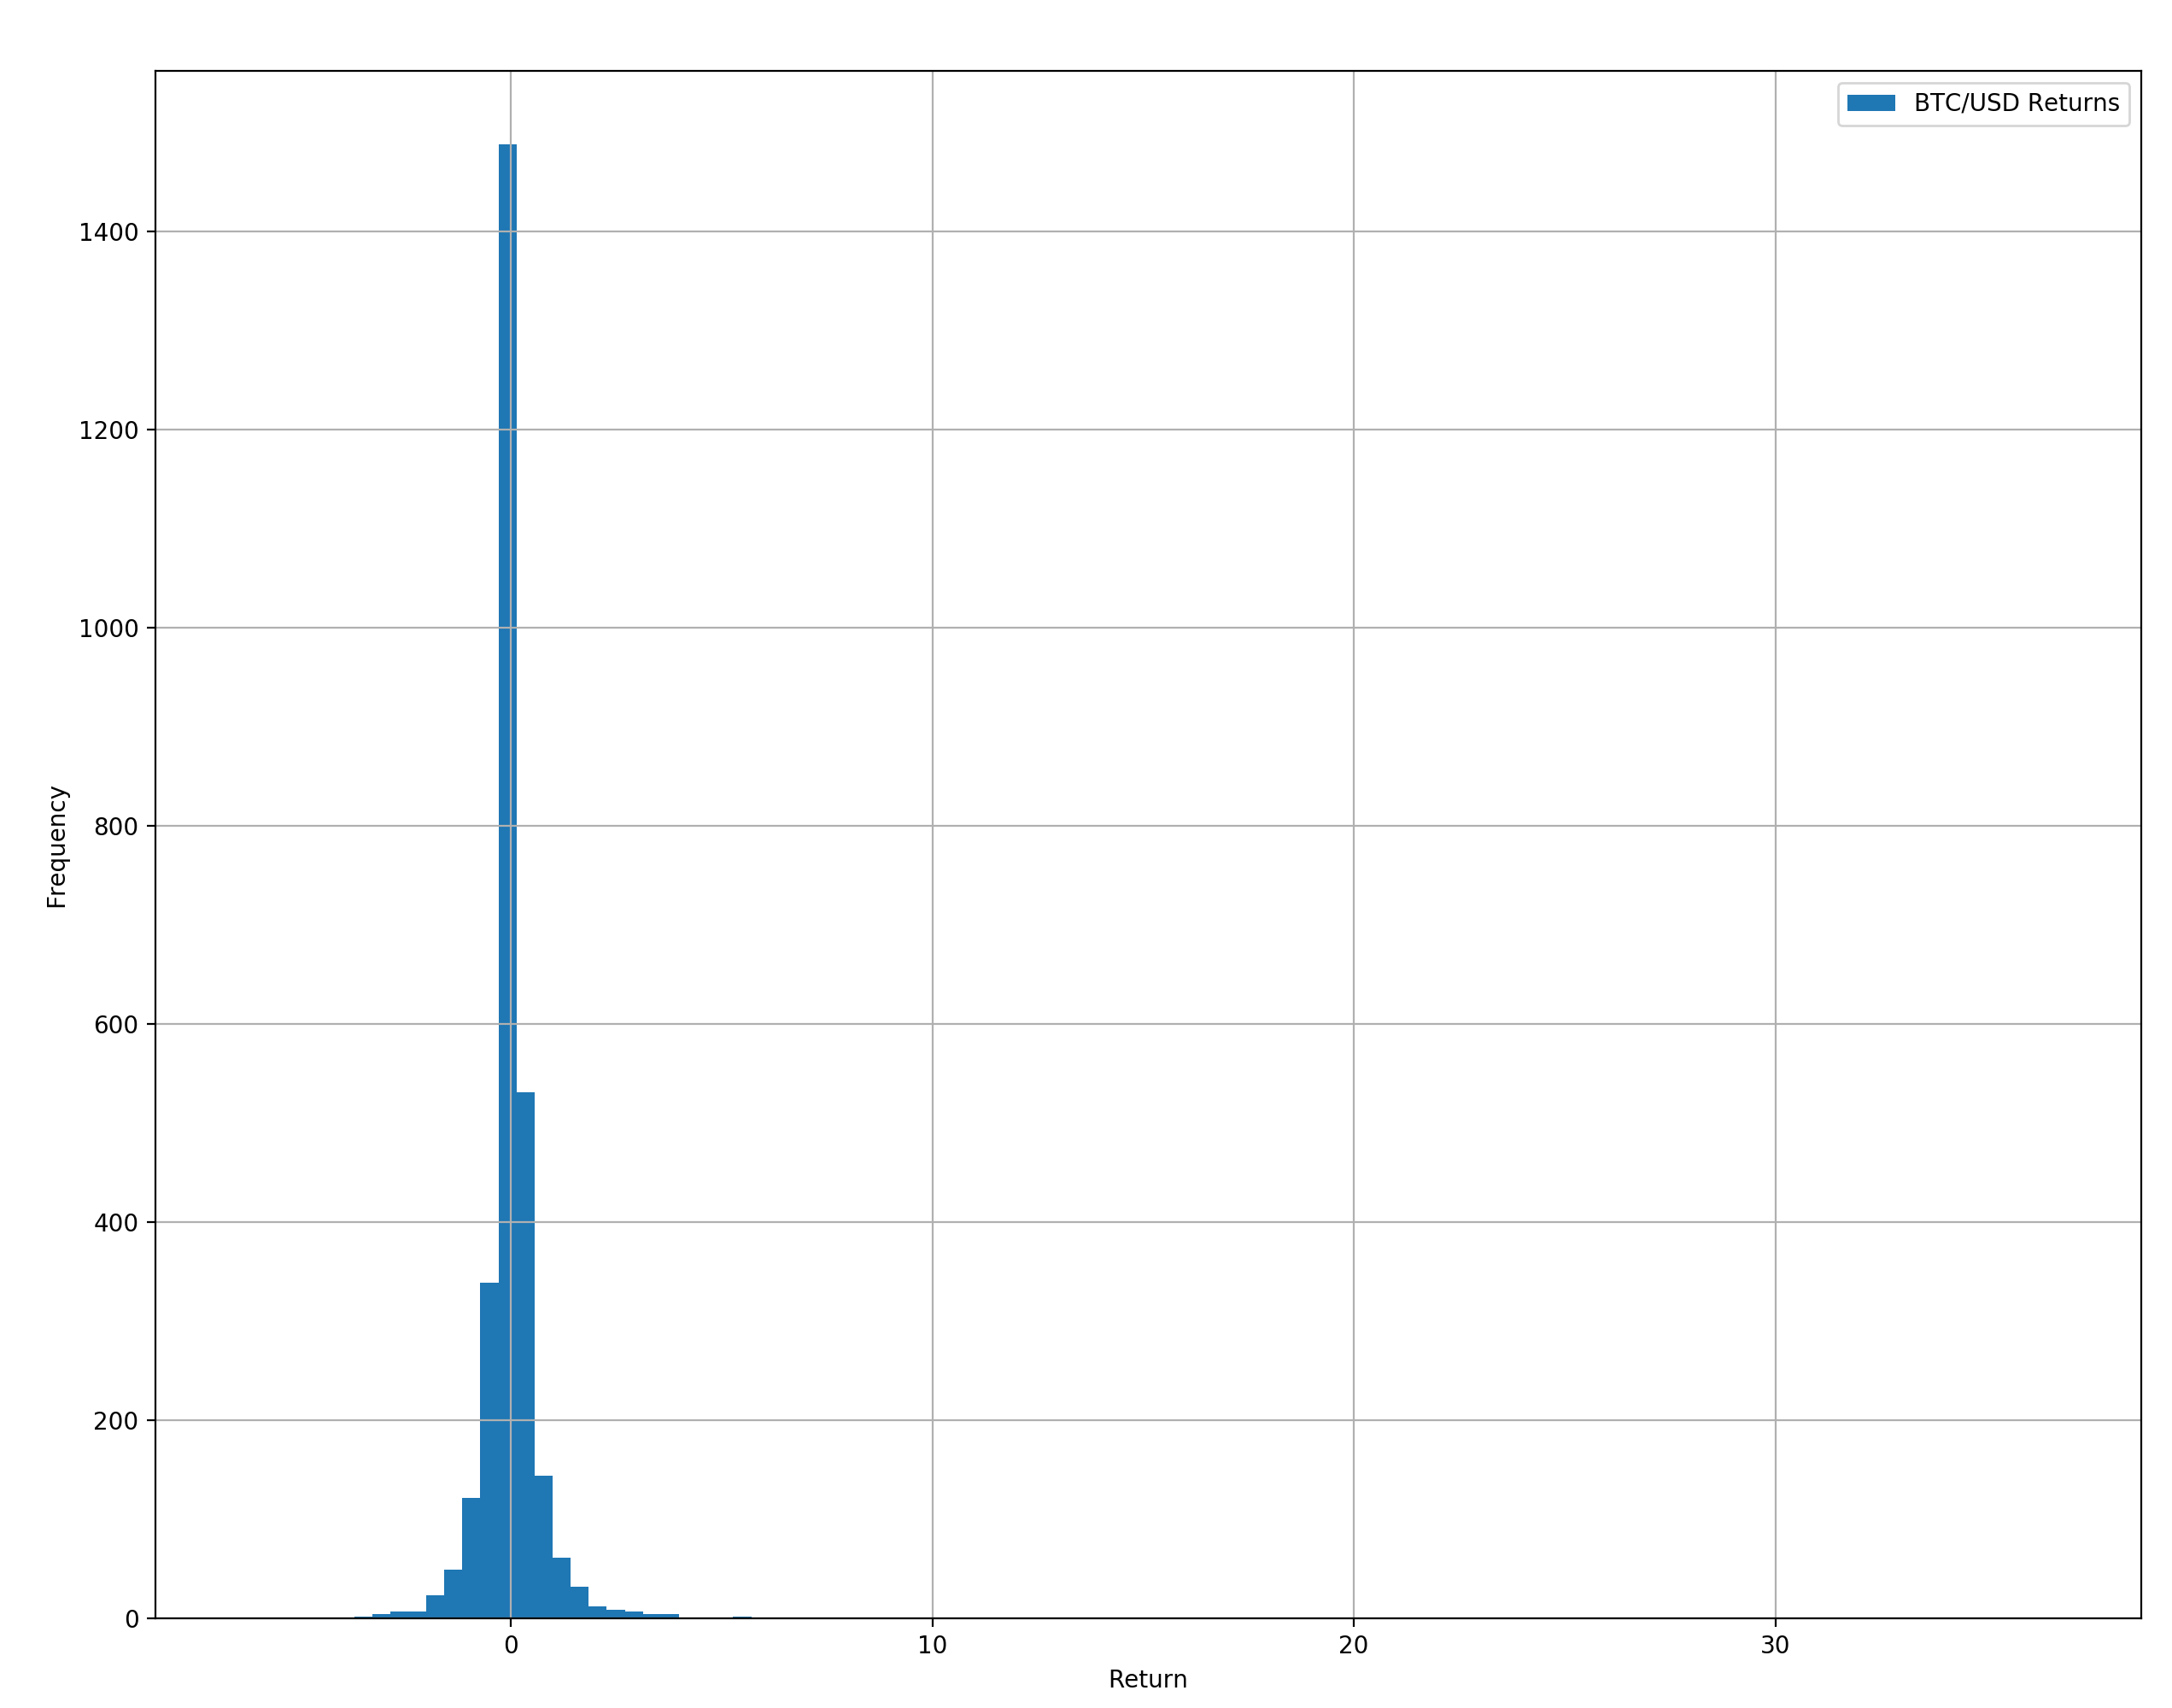
\includegraphics[width=\textwidth]{btc_returns_hist.png}
\end{figure}
\end{frame}

\begin{frame}
\frametitle{BTC/USD Daily Returns QQ-Plot (2010-2018)}
\begin{figure}[h!]
\centering 
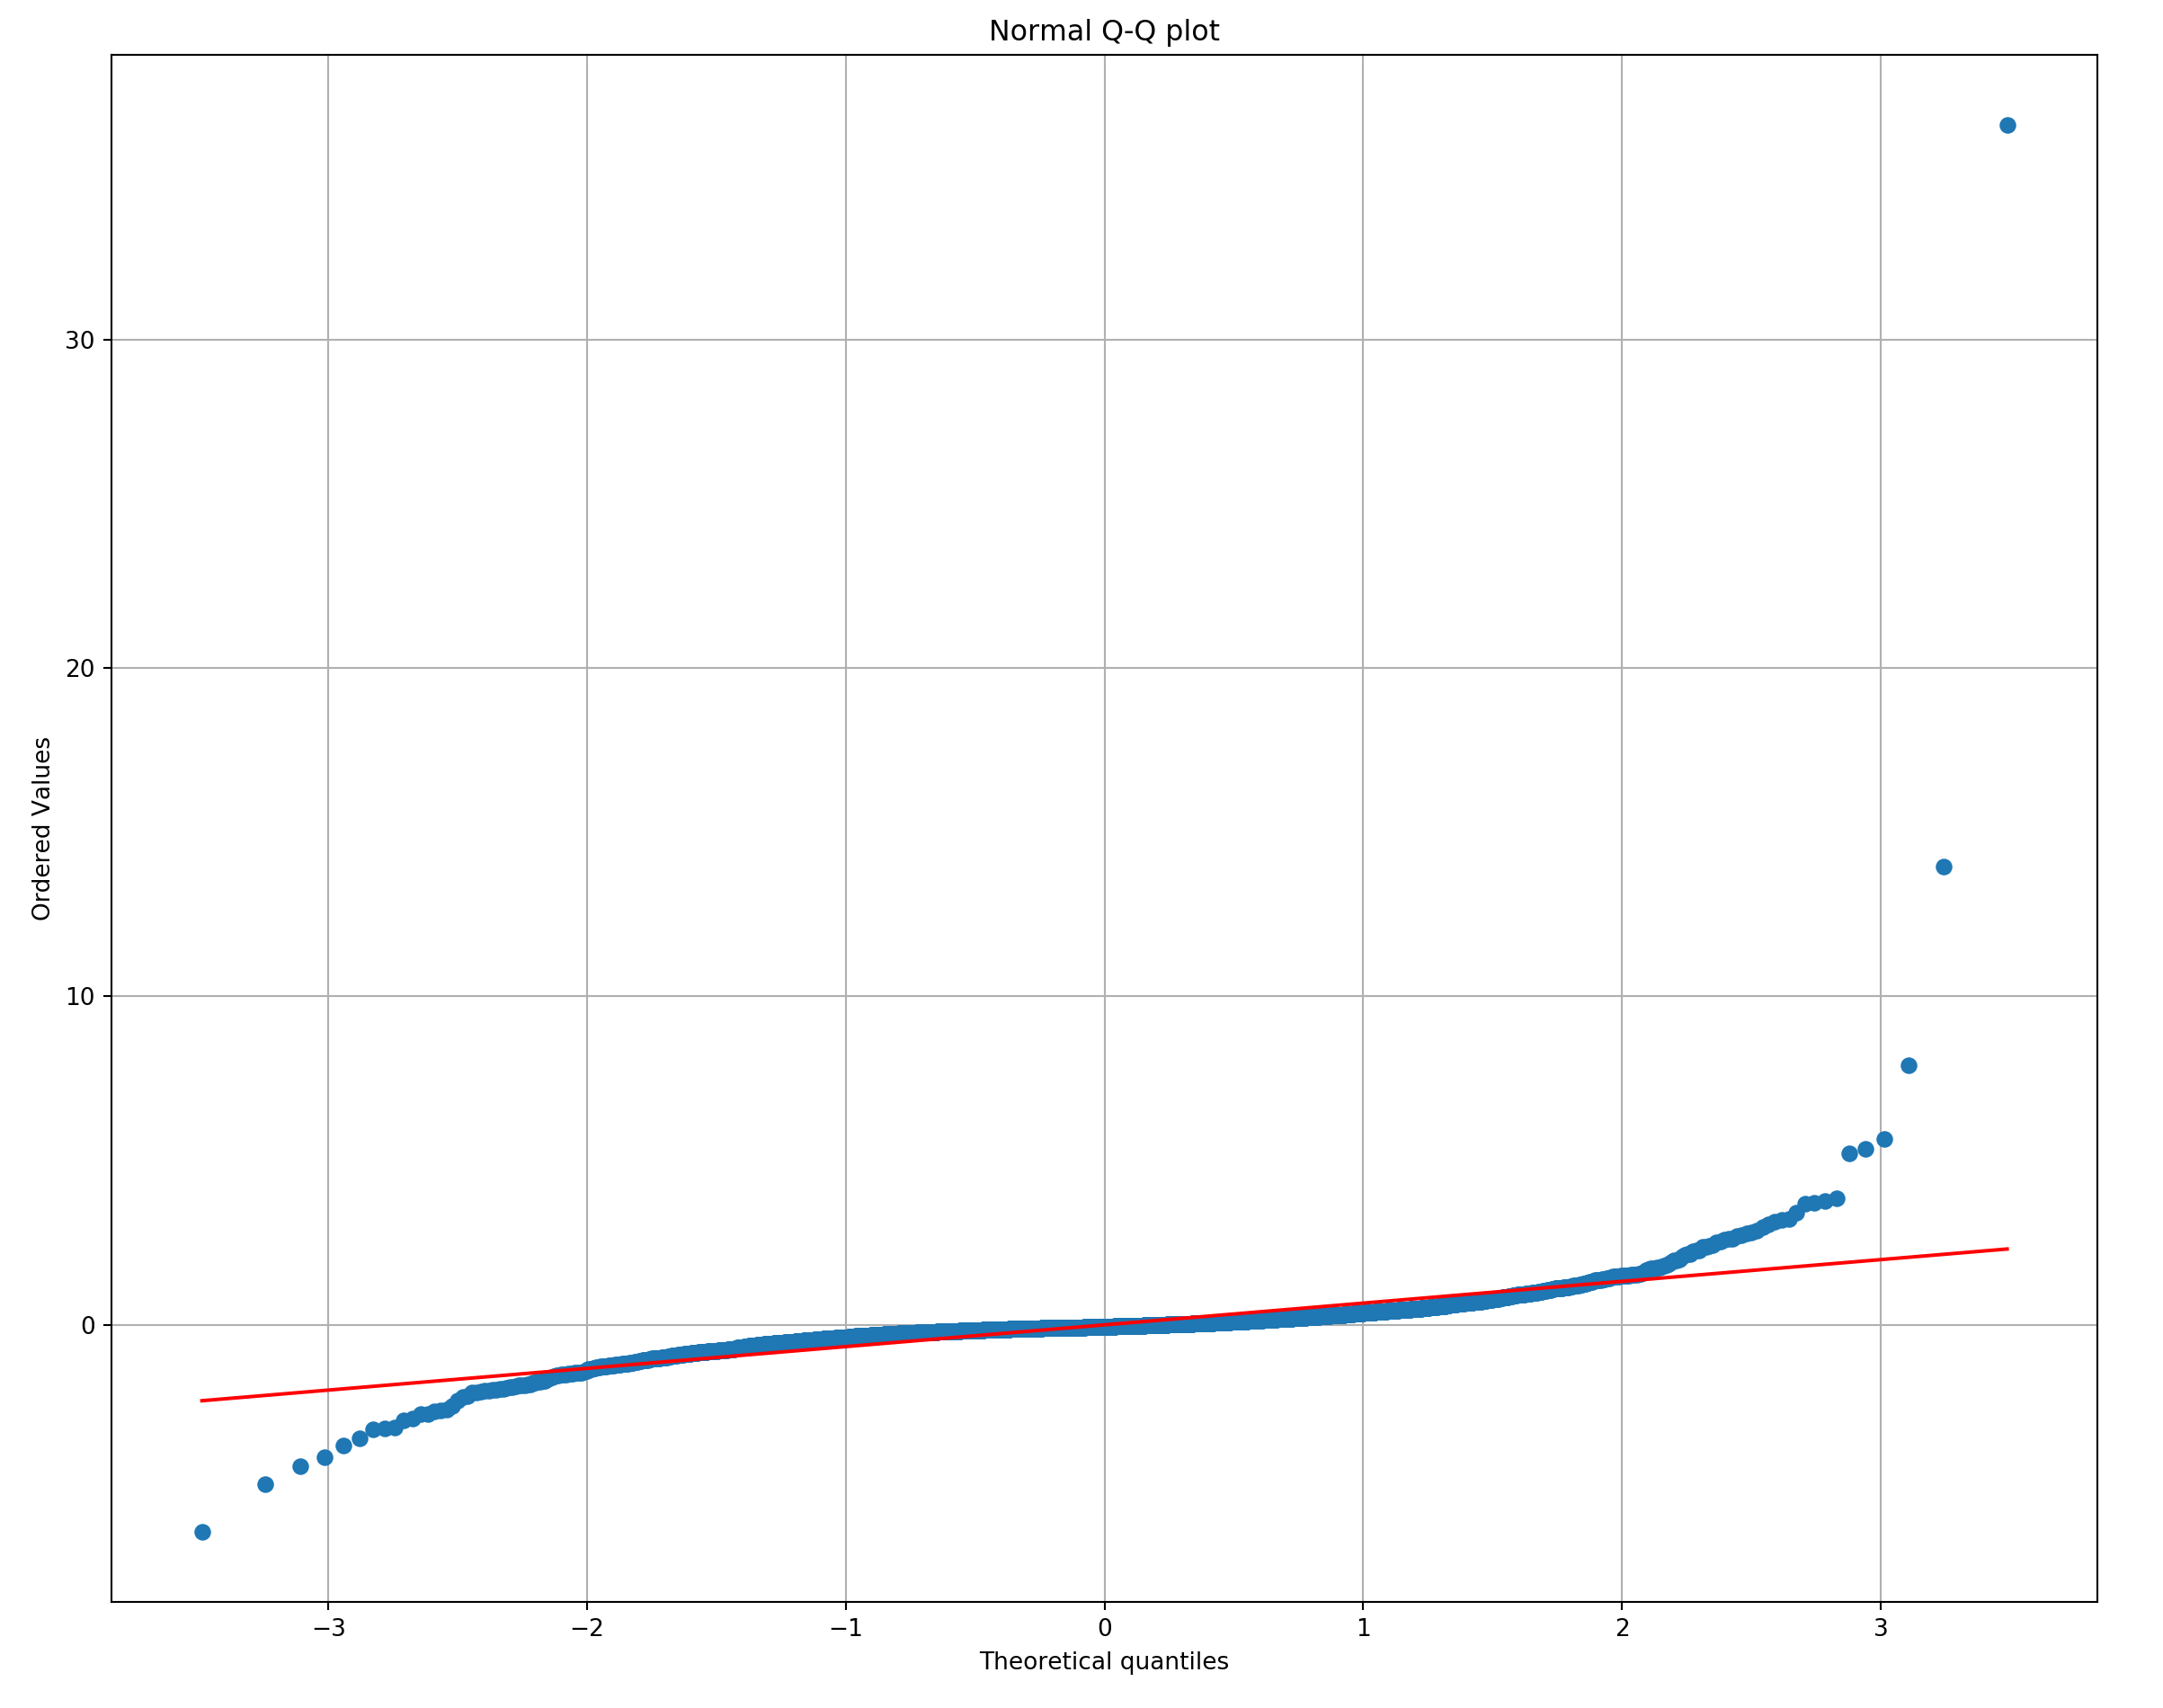
\includegraphics[width=\textwidth]{btc_returns_qqplot.png}
\end{figure}
\end{frame}

\begin{frame}
\frametitle{NoVaS Transformed BTC/USD Returns (p=12)}
\begin{figure}[h!]
\centering 
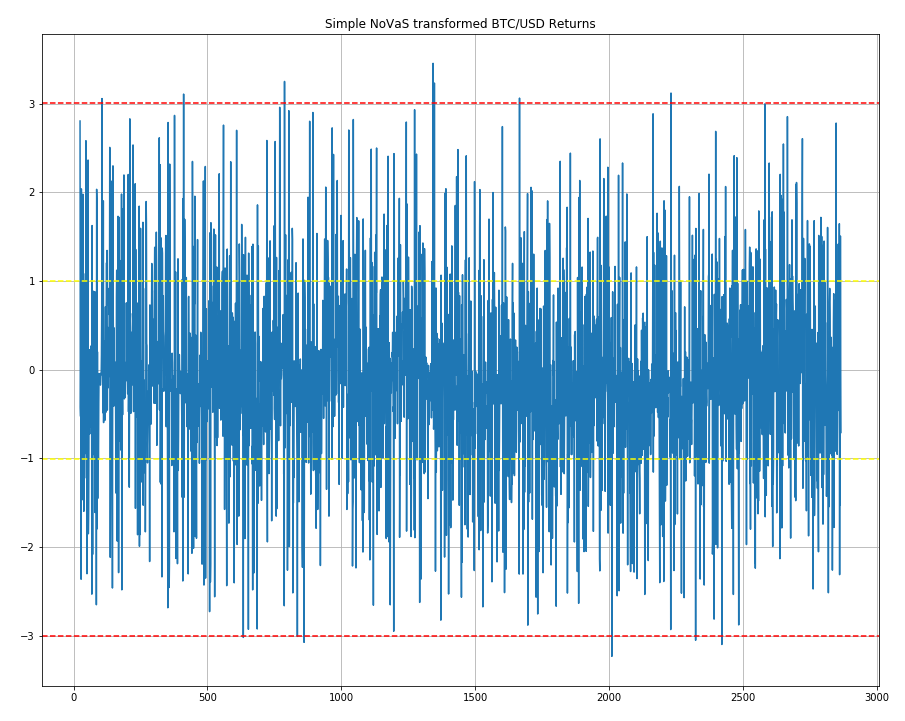
\includegraphics[width=\textwidth]{novas_btc_returns.png}
\end{figure}
\end{frame}

\begin{frame}
\frametitle{NoVaS Transformed BTC/USD Histogram (p=12)}
\begin{figure}[h!]
\centering 
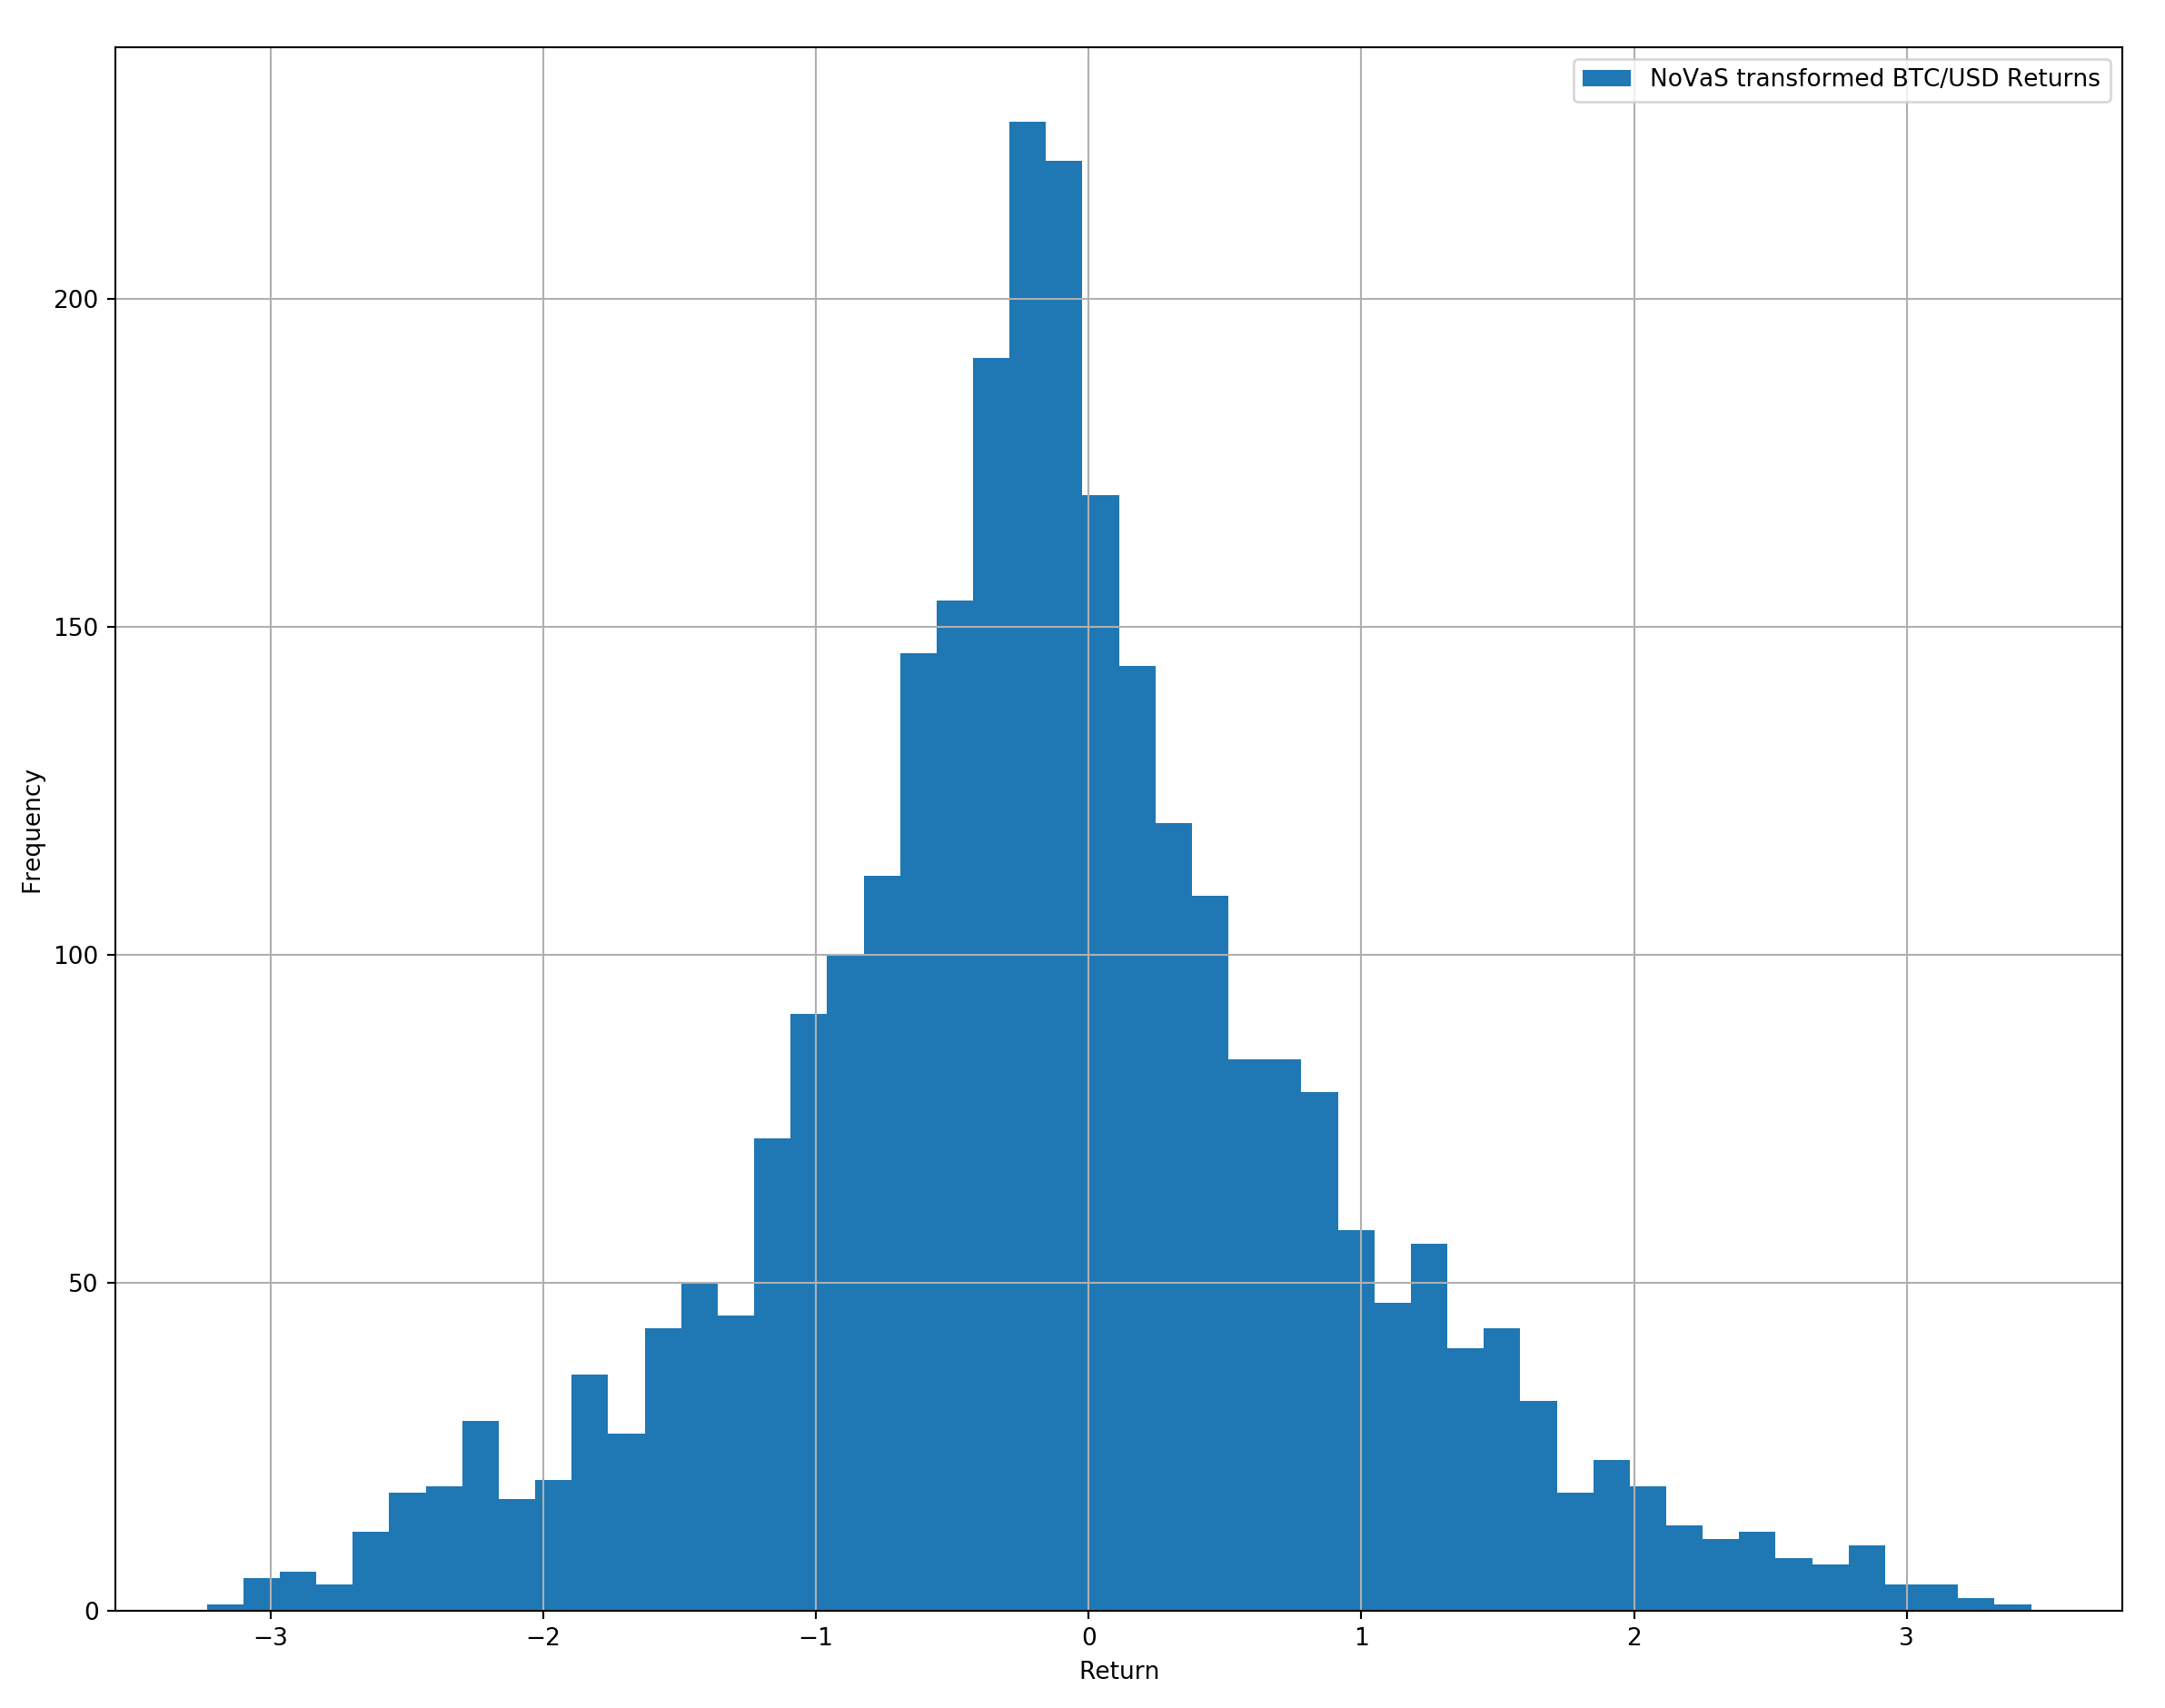
\includegraphics[width=\textwidth]{novas_btc_returns_hist.png}
\end{figure}
\end{frame}

\begin{frame}
\frametitle{NoVaS Transformed BTC/USD QQ-Plot (p=12)}
\begin{figure}[h!]
\centering 
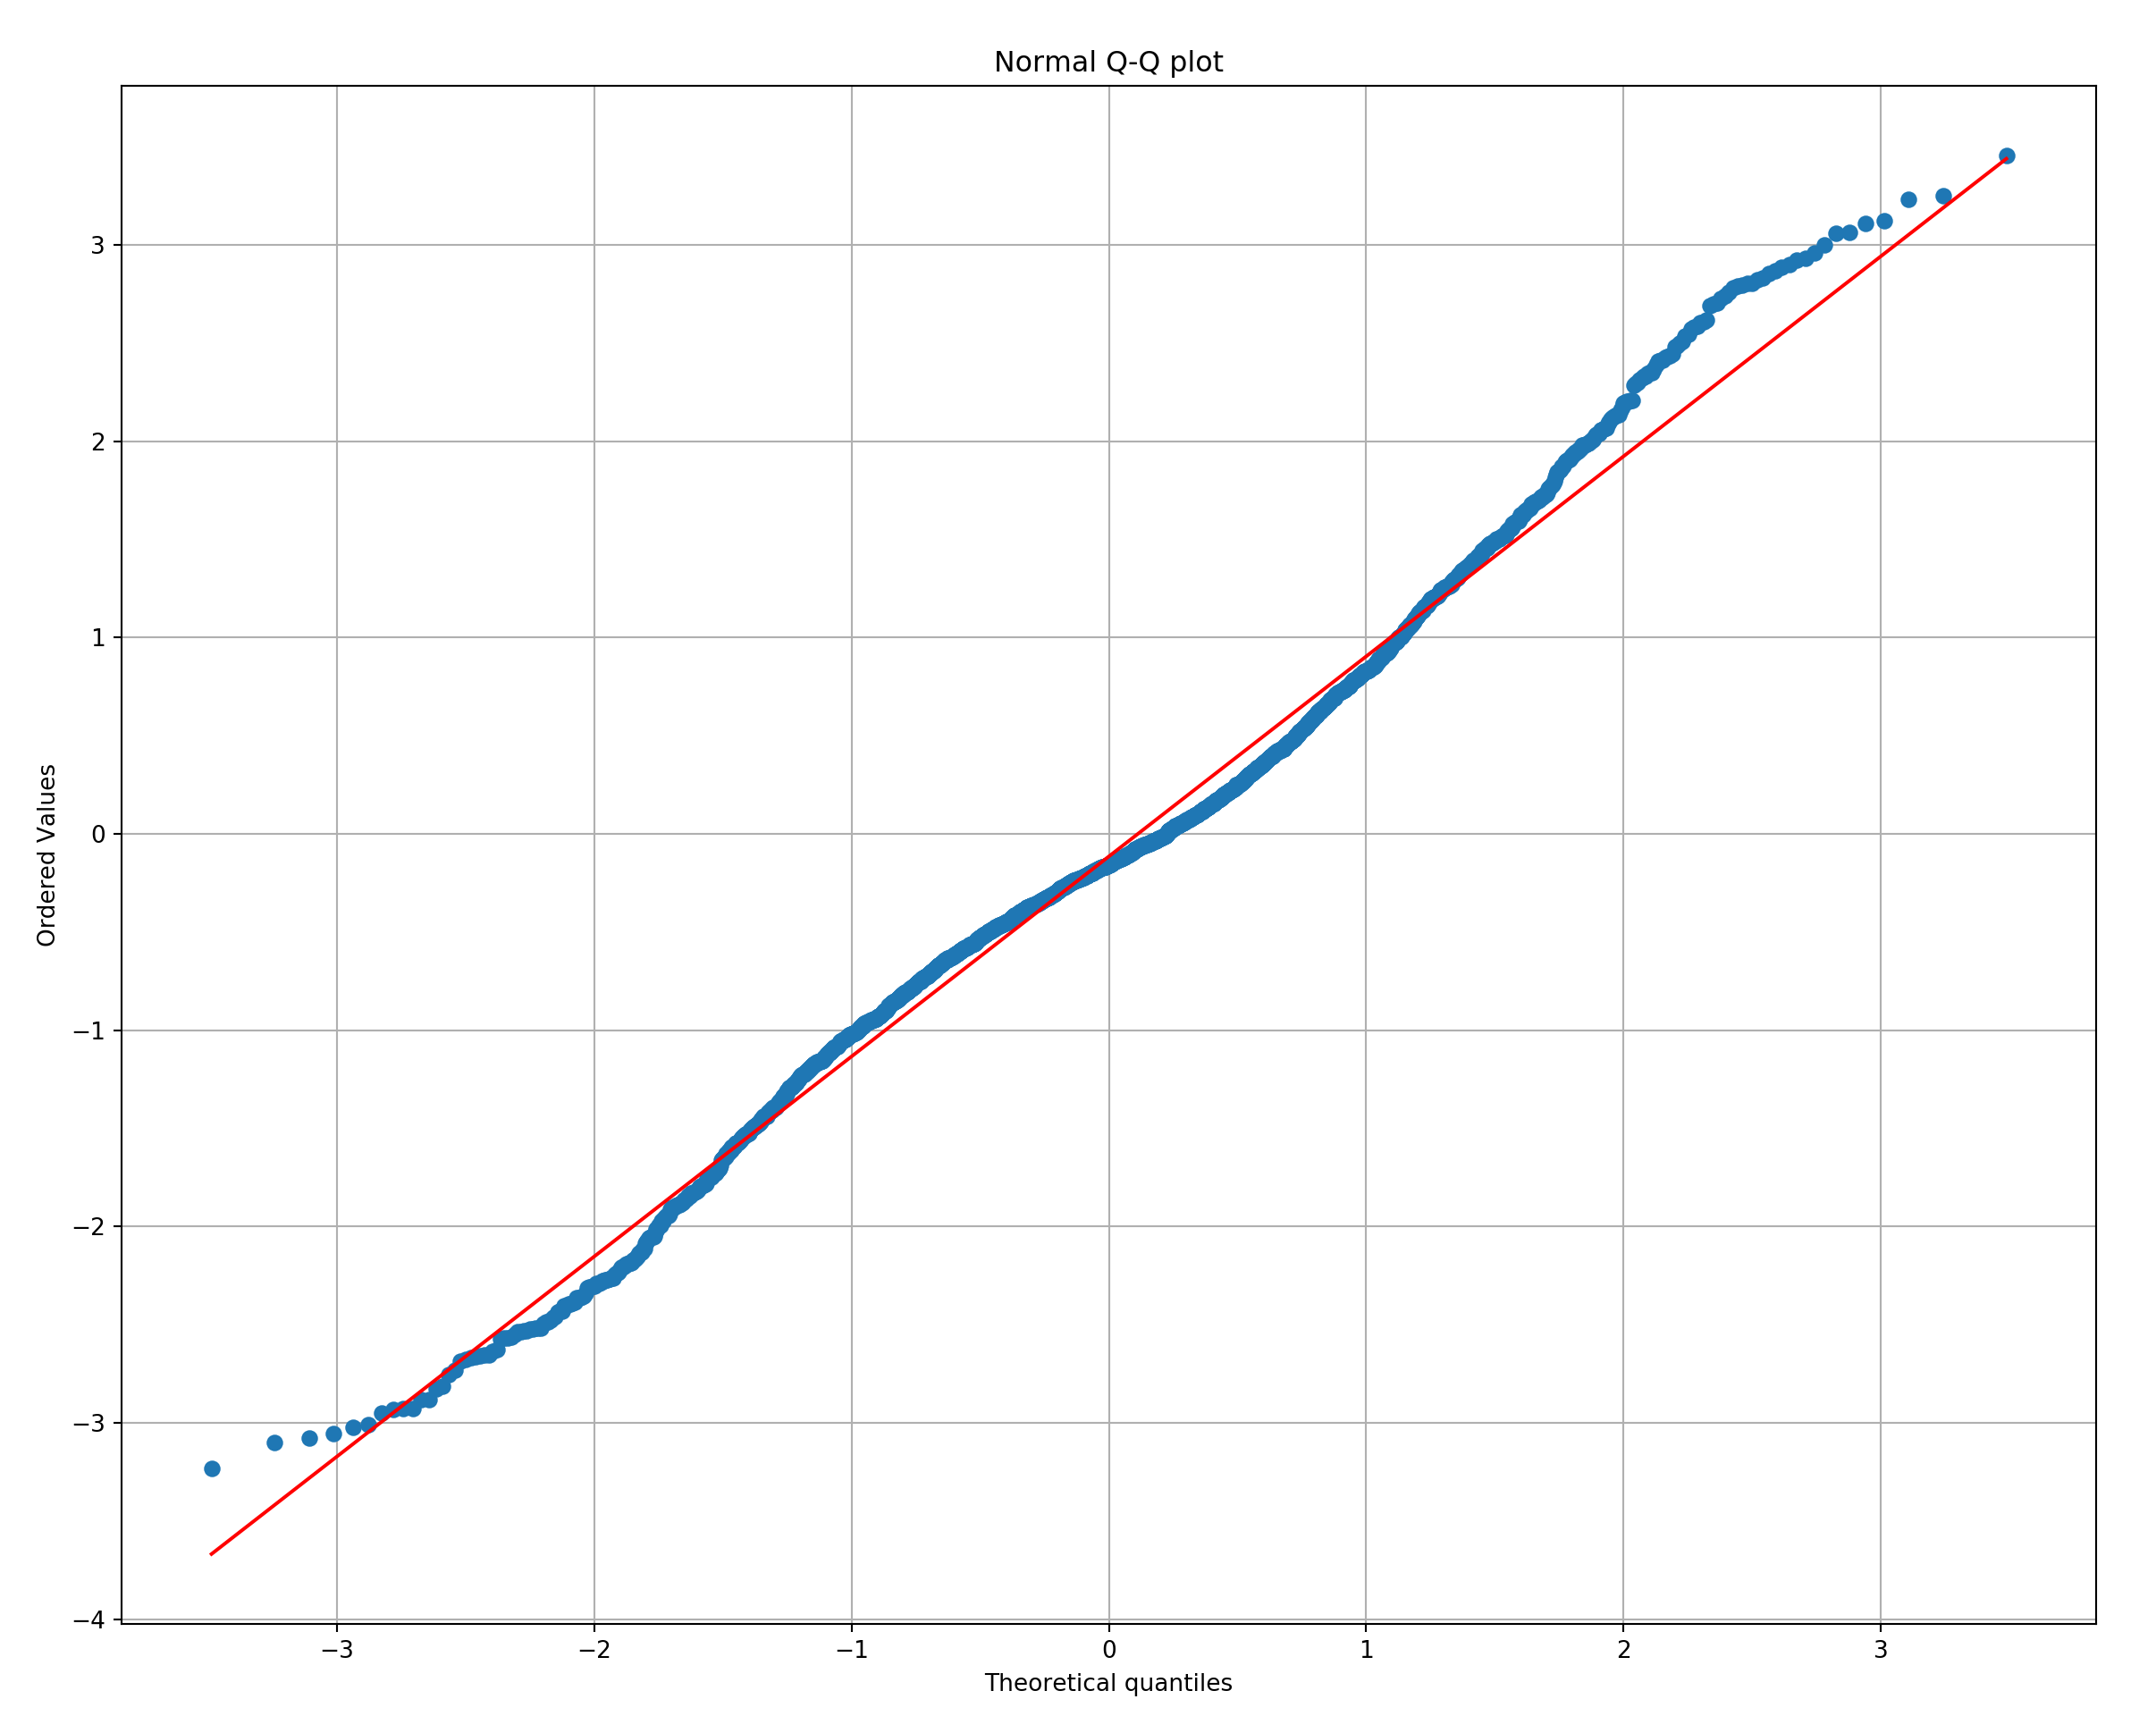
\includegraphics[width=\textwidth]{novas_btc_returns_qqplot.png}
\end{figure}
\end{frame}

%% 5 min bar US Treasury Futures 10 year %%
\begin{frame}
\frametitle{Treasury Futures}
pre-NoVas Treasury Futures returns plot
\end{frame}

\begin{frame}
\frametitle{Treasury Futures}
pre-NoVas Treasury Futures returns histogram
\end{frame}

\begin{frame}
\frametitle{Treasury Futures}
pre-NoVas Treasury Futures returns q-q plot
\end{frame}

\begin{frame}
\frametitle{Treasury Futures}
post-NoVas Treasury Futures returns plot
\end{frame}

\begin{frame}
\frametitle{Treasury Futures}
post-NoVas Treasury Futures returns histogram
\end{frame}

\begin{frame}
\frametitle{Treasury Futures}
post-NoVas Treasury Futures returns q-q plot
\end{frame}

\begin{frame}
\frametitle{S&P500 not perfect tranform with NoVaS}
Simply show an imperfect transformation to make the point that financial time series over long periods are not necessary stationary (only locally stationary) and thus we should use time-varying versions of NoVaS where the window size isn't too big.
\end{frame}


\section{Forecasting Volatility}

\begin{frame}
\frametitle{Outline}
\tableofcontents[currentsection]
\end{frame}

\begin{frame}
\frametitle{One-Step Ahead Prediction}
Define the volatility prediction problem.
Outline that you're using squared returns $Y_{t}^2$ as a noisy proxy for Volatility
What loss function should you use?
Will use a window size of 250 days which is approx. 1 year
\end{frame}

\begin{frame}
\frametitle{Infinite Kurtosis?}
Do financial returns have infinite kurtosis?
If this is the case you, predicting under L2 is incorrect. Instead you should L1 loss where the median is optimal
\end{frame}

\begin{frame}
\frametitle{Infinite Kurtosis Plot S&P500}

\end{frame}

\begin{frame}
\frametitle{Infinite Kurtosis Plot BTC}

\end{frame}

\begin{frame}
\frametitle{Infinite Kurtosis Plot Treasury Futures}

\end{frame}

\begin{frame}
\frametitle{Prediction Intervals}
Steps for deriving prediction intervals - same for GARCH and NoVaS
\end{frame}

\begin{frame}
\frametitle{S&P500 Feb 2018 One Step Ahead Prediction}
Plot predicting S&P500 Feb 2018 Volatility spike, along with prediction intervals
Shows that Simple NoVaS is better than GARCH(1,1)
\end{frame}

\section{A Simple Volatility Trading Strategy}

\begin{frame}
\frametitle{Outline}
\tableofcontents[currentsection]
\end{frame}

\begin{frame}
\frametitle{Can predict $sigma^2$ using NoVaS under special conditions}
Talk about the conditions under which you can actually predict $sigma^2$, plot the ACF to confirm that transformed series is uncorrelated and independent.
\end{frame}

\begin{frame}
\frametitle{RV(t+1)-IV(t)}
Outline strategy that if RV(t+1)-IV(t) $>$ 0 you buy VXX and vice versa.
\end{frame}

\begin{frame}
\frametitle{Strategy Results}
Cumulative returns plot, legend contains CAGR and Sharpe Ratio
\end{frame}

\end{document}